% 一个算例看懂耦合大小孔的 NMR：C3（w = 1 um，L = 15 um）的直观解读
% 配套 ../coupled_pore_backcalc.pdf（推导版）。图由 make_figures.py 生成；数值来自 ../numbers.json。
% 编译：xelatex c3_intuitive.tex（两次）
\documentclass[11pt,a4paper]{article}
\usepackage{xeCJK}
\setCJKmainfont[BoldFont=SimHei,ItalicFont=KaiTi]{Microsoft YaHei}
\setCJKsansfont{Microsoft YaHei}
\renewcommand{\tablename}{表}
\renewcommand{\figurename}{图}
\renewcommand{\refname}{参考文献}
\renewcommand{\contentsname}{目录}
\usepackage[margin=2.1cm]{geometry}
\usepackage{amsmath,amssymb}
\usepackage{siunitx}
\usepackage{booktabs}
\usepackage{array}
\usepackage{graphicx}
\usepackage{float}
\usepackage{enumitem}
\usepackage[round,semicolon]{natbib}
\setcitestyle{aysep={,}}
\usepackage{tcolorbox}
\usepackage[colorlinks=true,linkcolor=blue,citecolor=blue,urlcolor=blue]{hyperref}
\sisetup{per-mode=symbol,group-digits=false}
\graphicspath{{figures/}}
\urlstyle{same}
\setlength{\parskip}{3pt}

\newcommand{\Peff}{\Psi_{\mathrm{eff}}}
\newcommand{\TB}{T_{2B}}
\newcommand{\um}{\,\si{\micro m}}
\newcommand{\ms}{\,\si{ms}}
\newcommand{\pms}{\,\si{ms^{-1}}}

% four box types used throughout: picture -> formula -> numbers -> takeaway
\newtcolorbox{intuit}[1][]{colback=orange!5,colframe=orange!55!black,fonttitle=\bfseries,
  title={形象理解#1},left=6pt,right=6pt,top=4pt,bottom=4pt}
\newtcolorbox{formula}[1][]{colback=blue!3,colframe=blue!45!black,fonttitle=\bfseries,
  title={公式与每一项的物理意义#1},left=6pt,right=6pt,top=4pt,bottom=4pt}
\newtcolorbox{numbers}[1][]{colback=gray!5,colframe=gray!55!black,fonttitle=\bfseries,
  title={代入 C3 的数值#1},left=6pt,right=6pt,top=4pt,bottom=4pt}
\newtcolorbox{takeaway}[1][]{colback=green!4,colframe=green!40!black,fonttitle=\bfseries,
  title={从这一步读出什么#1},left=6pt,right=6pt,top=4pt,bottom=4pt}
\newtcolorbox{pitfall}[1][]{colback=red!3,colframe=red!50!black,fonttitle=\bfseries,
  title={#1},left=6pt,right=6pt,top=4pt,bottom=4pt}

\title{一个算例看懂耦合大小孔的 NMR\\[3pt]
\large C3（喉宽 $w=1\um$，喉长 $L=15\um$）的直观解读}
\author{}
\date{配套文档：\texttt{coupled\_pore\_backcalc.pdf}（推导版）}

\begin{document}
\maketitle

\noindent\textbf{这份文档怎么读。}
只看一个算例 C3，从你已经熟悉的“水分子乱跑、碰壁被消磁”出发，一步一步加入喉道的作用，直到解释清楚 C3 的 $T_2$ 谱为什么长这样、直接换算孔径为什么会错、怎样纠正。
每一步都按同一个顺序：\textbf{形象理解 → 公式（只讲每一项的意思，不推导）→ 代入 C3 的数值 → 读出什么}。
完整推导、20 个算例的分区判据和参考文献见推导版。

\noindent\textbf{数值的来源。}
几何和物理参数是模拟设定值；“模拟 + NNLS”的峰位和面积来自已经完成的全二维有限元模拟与 L-curve NNLS 反演；
标为“手算”的数值来自一个简化模型（准静态两点交换），用来帮助理解，与精确模型相差约 5\%。全部结果为\textbf{二维}模型（每单位纵深）。

\begin{tcolorbox}[colback=yellow!6,colframe=yellow!45!black,fonttitle=\bfseries,title={先看结论：C3 的 $T_2$ 谱告诉了我们什么}]
\begin{enumerate}[leftmargin=1.6em,itemsep=2pt]
\item 谱上能看到两个峰，但\textbf{小孔峰在 215\ms}，而一个孤立的 5\um 小孔应在约 441\ms；\textbf{小孔峰的面积只有应有值的 39\%}。
\item 主峰在 1087\ms，而孤立的 20\um 大孔应在约 1206\ms——\textbf{大孔峰也被拉短了}。
\item 原因是喉道同时扮演两个角色：\textbf{“下水道”}（喉道壁把进来的磁化消掉）和\textbf{“走廊”}（两孔的水互相交换）。
\item 用孤立孔公式直接换算：小孔 2.31\um（真值 5）、大孔 17.04\um（真值 20）。
\item 衡量“走廊”强弱的数 $\Peff=0.61$，C3 处在“过渡区”：两峰都还在，但都被拉偏了。
\item 如果另外知道喉道尺寸（CT 或 SIP），可以用模型把偏移“扣除”，得到 4.84\um 和 19.61\um。
\end{enumerate}
\end{tcolorbox}

\tableofcontents

%==========================================================================
\section{C3 是什么样的体系}

\begin{figure}[H]
\centering
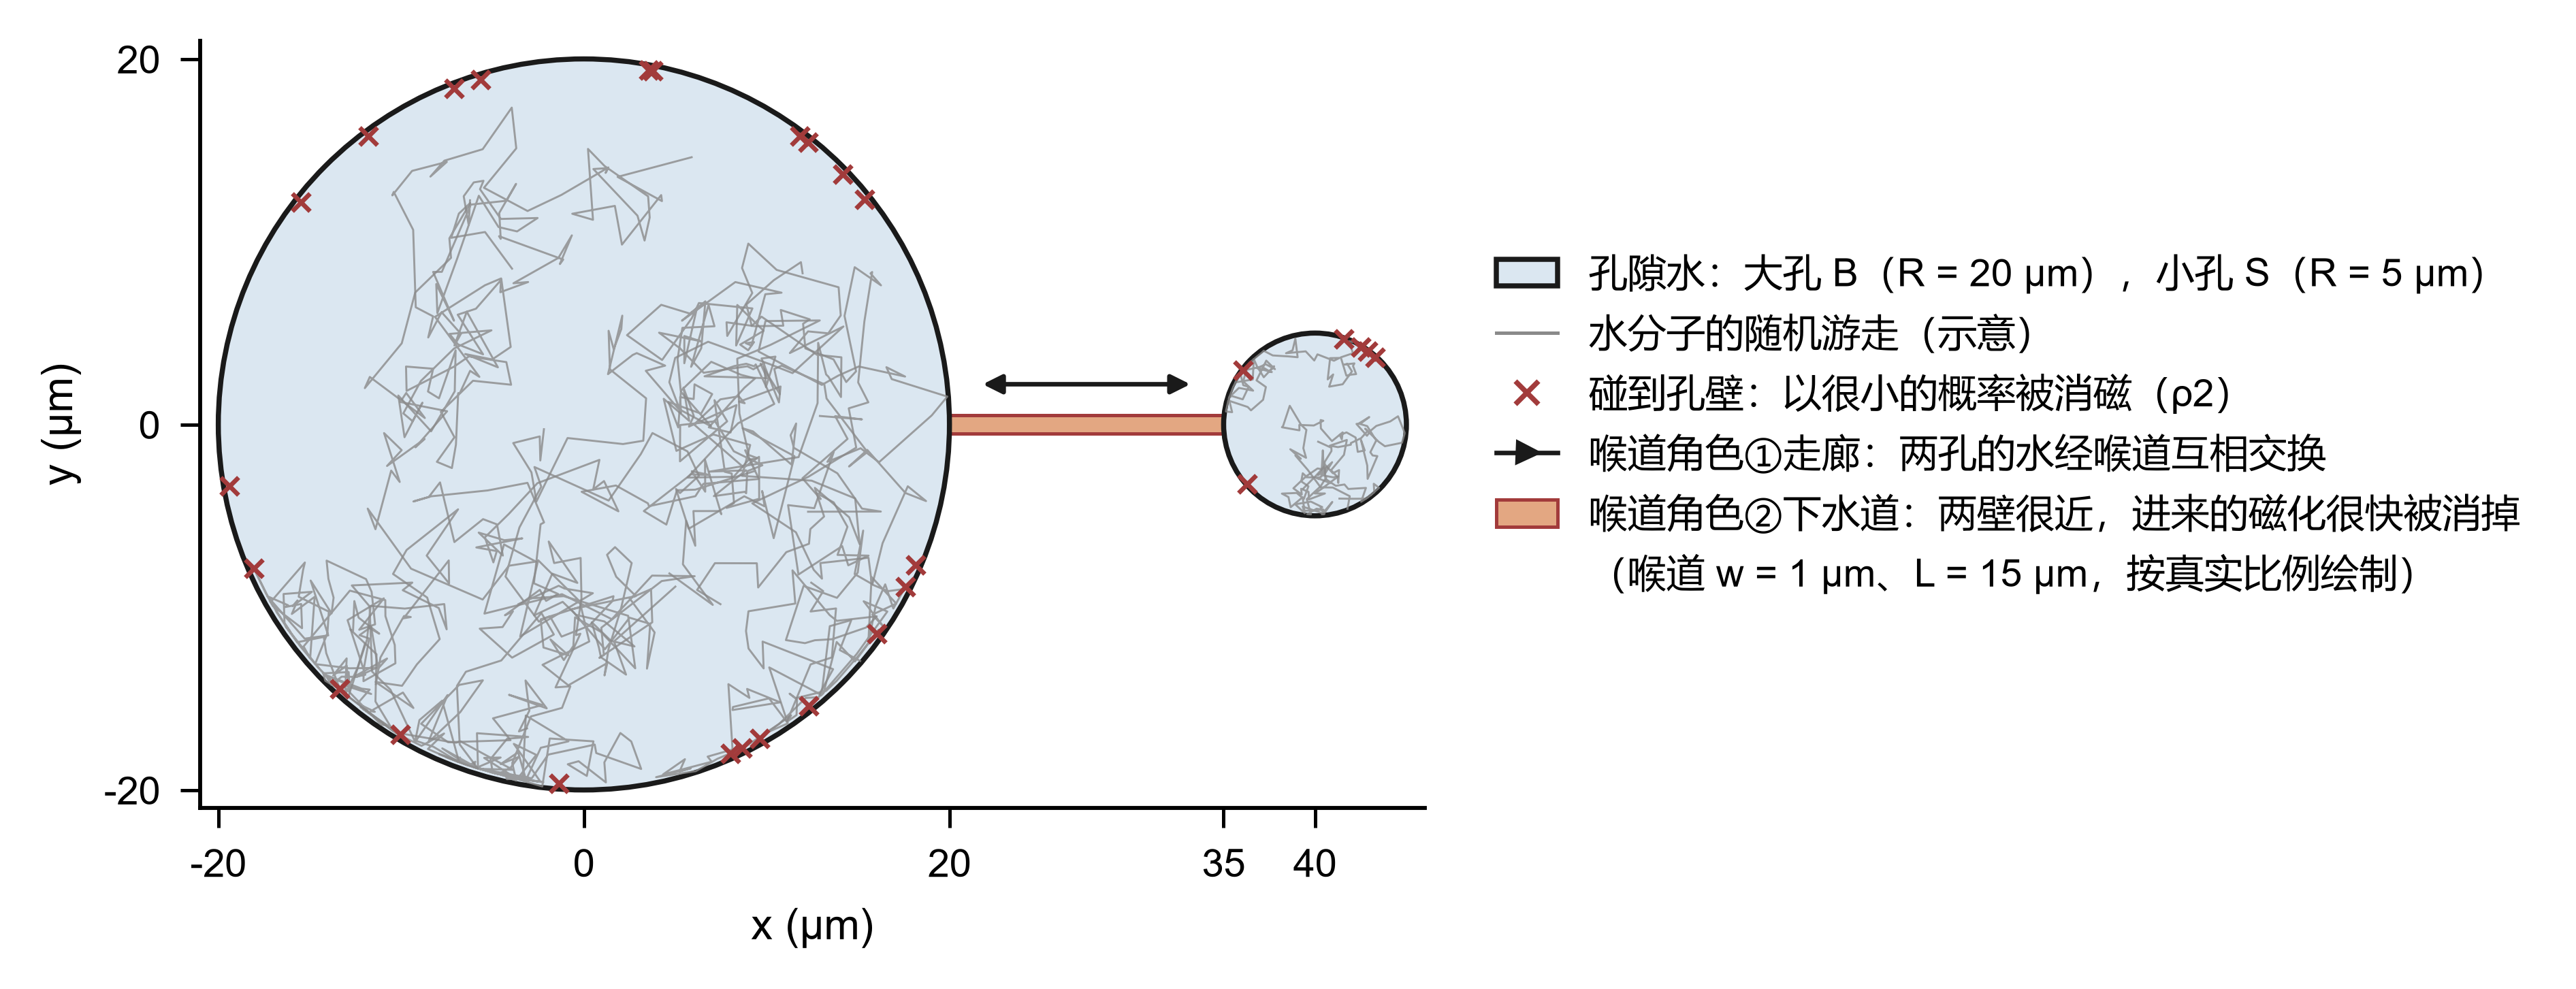
\includegraphics[width=\textwidth]{fig_c3_schematic.png}
\caption{C3 的几何（按真实比例）与三件同时发生的事：水分子在孔内随机游走、碰到孔壁时以很小的概率被消磁；喉道一方面让两孔的水互相交换（走廊），
另一方面它的两壁相距只有 1\um，进入喉道的磁化很快被消掉（下水道）。随机游走轨迹和碰壁位置只是示意。}
\label{fig:schematic}
\end{figure}

\begin{table}[H]
\centering\small
\caption{C3 的设定参数及其通俗含义。}
\label{tab:params}
\begin{tabular}{@{}l l l@{}}
\toprule
量 & 数值 & 通俗含义 \\
\midrule
$D$ & $2.0\,\si{\micro m^2/ms}$ & 水分子“乱跑”的快慢（自扩散系数） \\
$\rho_2$ & $0.005\,\si{\micro m/ms}$（$5\,\si{\micro m/s}$） & 孔壁“消磁能力”：每碰一次壁，有一定概率被消磁 \\
$\TB$ & 3000\ms & 不碰壁时水自身的“自然寿命”（体弛豫） \\
大孔 B & 半径 20\um，面积 $A_B=1256.6\,\si{\micro m^2}$ & 水多、墙相对少 \\
小孔 S & 半径 5\um，面积 $A_S=78.54\,\si{\micro m^2}$ & 水少、墙相对多；占总孔隙面积 $p_S=5.88\%$ \\
喉道 & 宽 $w=1\um$，长 $L=15\um$ & 连接两孔的细长通道 \\
\bottomrule
\end{tabular}
\end{table}

%==========================================================================
\section{第一步：一个孤立的孔——你已经熟悉的图像}

\begin{intuit}
把孔想成一个房间，水分子是房间里到处乱走的人，墙上贴着“消磁贴纸”。一个人每碰一次墙，就有很小的概率失去磁化。
房间越大，每个人平均要走得越久才能碰到墙，所以\textbf{大孔弛豫慢、小孔弛豫快}。
关键不在于“孔大”本身，而在于\textbf{每一份水对应多少墙}。
\end{intuit}

\begin{formula}
\begin{equation}
\frac{1}{T_2}=\rho_2\,\frac{P}{A}+\frac{1}{\TB}
\label{eq:single}
\end{equation}
\begin{itemize}[leftmargin=1.4em,itemsep=1pt]
\item $P/A$：孔壁长度 $P$ 除以孔面积 $A$（二维），即“每单位水对应多少墙”。圆孔 $P/A=2/R$。
\item $\rho_2 P/A$：墙造成的消磁速率 = 墙的“杀伤力” × 墙的“多少”。
\item $1/\TB$：不碰墙也会发生的慢速消磁，这里 3000\ms，比孔壁作用慢得多。
\end{itemize}
把式 \eqref{eq:single} 反过来用，就是从 $T_2$ 读孔径的\textbf{“尺子”}（二维圆孔）：
\begin{equation}
r=\frac{2\rho_2}{1/T_2-1/\TB}.
\label{eq:ruler}
\end{equation}
这把尺子是按“孤立孔”刻度的。后面会看到，孔一旦被喉道连起来，尺子就会读错。
\end{formula}

\begin{formula}[：什么时候可以把一个孔当作“一个点”]
上面的公式成立的前提是\textbf{孔内的磁化处处均匀}。这需要水分子跑遍整个孔所用的时间 $R^2/D$，远短于孔的 $T_2$。
等价地，用无量纲数 $\kappa=\rho_2R/D$ 衡量：$\kappa\ll1$ 表示分子要碰很多次墙才会被消磁，孔内来得及混匀。
\end{formula}

\begin{numbers}
\begin{itemize}[leftmargin=1.4em,itemsep=1pt]
\item 小孔：$P_S/A_S=30.41/78.54=0.387\,\si{\micro m^{-1}}$，$1/T_2=0.005\times0.387+1/3000=2.270\times10^{-3}\pms$，$T_2=441\ms$。
\item 大孔：$P_B/A_B=124.66/1256.6=0.0992\,\si{\micro m^{-1}}$，$1/T_2=8.29\times10^{-4}\pms$，$T_2=1206\ms$。
\item 跑遍全孔的时间：小孔 $R^2/D=25/2=12.5\ms\ll441\ms$；大孔 $400/2=200\ms\ll1206\ms$。$\kappa$ 分别为 0.0125 和 0.05。
\end{itemize}
（喉口那 1\um 宽的开口不是墙，所以 $P$ 比完整圆周 $2\pi R$ 略短；用尺子 \eqref{eq:ruler} 读出的孤立小孔、大孔半径为 5.16\um 和 20.16\um，比 5 和 20 略大。）
\end{numbers}

\begin{takeaway}
\begin{itemize}[leftmargin=1.4em,itemsep=1pt]
\item 两个孔各自都满足“快扩散”，所以可以把每个孔看成一个磁化均匀的“水池”，只用一个数（池内平均磁化）描述它。
\item 如果两孔互不相连，谱上应有两个峰：约 441\ms（小孔，面积 5.9\%）和约 1206\ms（大孔，面积 94.1\%）。
C3 实测的 215\ms 和 1087\ms 都偏离了这两个值，下面解释原因。
\end{itemize}
\end{takeaway}

%==========================================================================
\section{第二步：加上喉道——它同时是“走廊”和“下水道”}

\subsection{喉道里的水消磁特别快}

\begin{intuit}
喉道是一条宽 1\um 的窄缝，两面墙几乎贴在一起。水分子在里面走两步就撞墙，所以喉道里的水消磁极快。
任何从孔里扩散进喉道的磁化，都很可能在喉道里被消掉——这就是\textbf{“下水道”}。
\end{intuit}

\begin{formula}
\begin{equation}
R_t=\frac{\rho_2}{h}+\frac{1}{\TB},\qquad h=\frac{w}{2}
\end{equation}
和式 \eqref{eq:single} 是同一个意思：窄缝的 $P/A=2/w=1/h$。$R_t$ 是喉道里的消磁速率，$1/R_t$ 是喉道里的“寿命”。
\end{formula}

\begin{numbers}
喉道 $P/A=2/1=2\,\si{\micro m^{-1}}$，是小孔（0.387）的 5 倍、大孔（0.099）的 20 倍。
$R_t=0.005/0.5+1/3000=0.01033\pms$，即喉道里的水约 \textbf{97\ms} 就基本消磁，比小孔（441\ms）快 4.5 倍。
\end{numbers}

\subsection{关键尺度：分子在喉道里“活着”能走多远}

\begin{intuit}
扩散的规律是：走过的距离 $\approx\sqrt{D\times\text{时间}}$。分子在喉道里的“寿命”约为 $1/R_t$，所以它活着时能走的距离是
$\ell=\sqrt{D/R_t}$。拿喉道长度 $L$ 和 $\ell$ 比一比：
\begin{itemize}[leftmargin=1.4em,itemsep=1pt]
\item $L\ll\ell$（短喉道）：分子轻松穿过，喉道是一条\textbf{畅通的走廊}；
\item $L\gg\ell$（长喉道）：分子走不到对面就“阵亡”，喉道只剩\textbf{两端的下水道口}，两孔基本互不来往；
\item $L\approx\ell$：两种作用都明显。
\end{itemize}
\end{intuit}

\begin{formula}
\begin{equation}
q=\frac{1}{\ell}=\sqrt{\frac{R_t}{D}},\qquad qL=\frac{L}{\ell}=\frac{\text{喉道长度}}{\text{分子在喉道里的“寿命行程”}}.
\end{equation}
$qL$ 是描述喉道性格的唯一数：$qL\ll1$ 偏“走廊”，$qL\gg1$ 偏“下水道”。
\end{formula}

\begin{numbers}
$\ell=\sqrt{2/0.01033}=13.9\um$，$q=0.0719\,\si{\micro m^{-1}}$；网格中喉道壁到壁长度 $L=15.03\um$，所以 $qL=1.08$。
C3 的喉道长度刚好约等于分子的“寿命行程”，\textbf{两种作用都不能忽略}。
\end{numbers}

\begin{figure}[H]
\centering
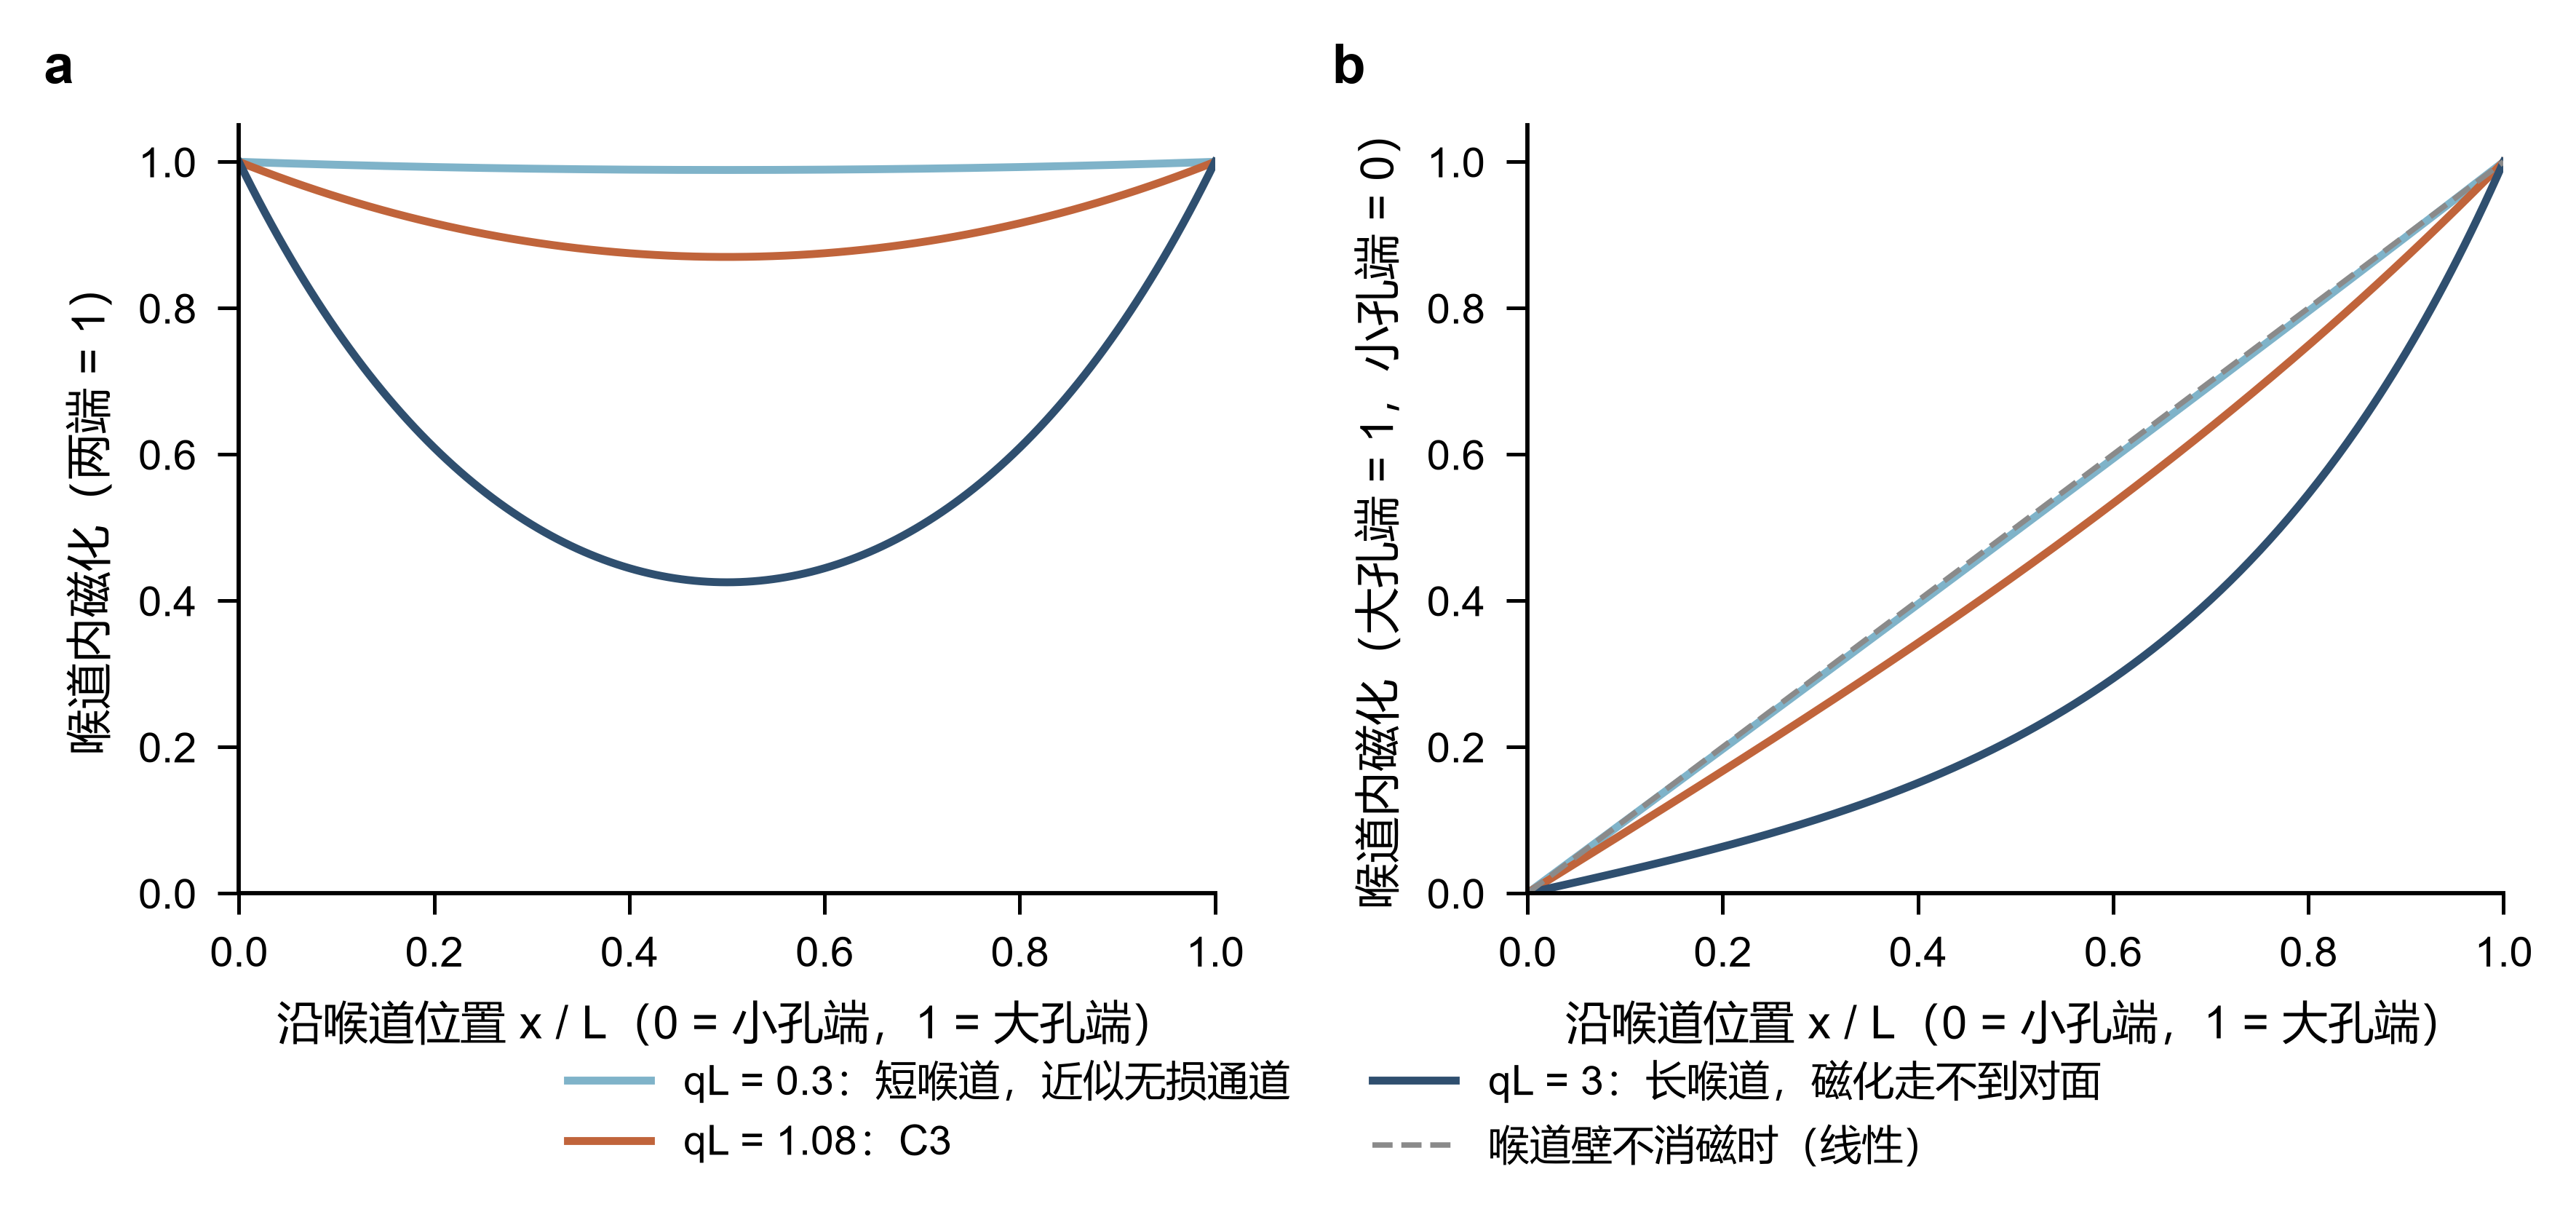
\includegraphics[width=\textwidth]{fig_c3_throat_profile.png}
\caption{$qL$ 的直观含义：喉道内磁化沿长度的分布。
(a) 两端都是满磁化（=1）时，喉道中间被“下水道”吃掉的程度：C3（$qL=1.08$）中点只剩 0.87；长喉道（$qL=3$）只剩 0.43。
(b) 只有大孔一端有磁化时，磁化沿喉道向小孔端传递；虚线是喉道壁不消磁时的直线分布，曲线越往下弯，路上损失越多。}
\label{fig:throat}
\end{figure}

\subsection{图~\ref{fig:throat} 是怎么画出来的：喉道里的“收支平衡”}
\label{sec:throat-balance}

图~\ref{fig:throat} 不是数值模拟的结果，而是由一个解析公式直接画出来的。这个公式来自喉道里每一小段的“收支平衡”。

\begin{intuit}
把喉道切成很多很薄的小片，盯住其中一片：
\begin{itemize}[leftmargin=1.4em,itemsep=1pt]
\item \textbf{收入}：两侧相邻小片的磁化扩散进来。磁化从多的地方流向少的地方，就像热从高温流向低温。
\item \textbf{支出}：这一片里的水碰到两面墙被消磁。
\end{itemize}
喉道又细又短，分子在里面约 97\ms 就“阵亡”，内部分布调整得很快，可以近似认为任何时刻都已经“收支平衡”：
\textbf{扩散送进来多少，墙就吃掉多少}（准静态近似）。

\textbf{工程类比——散热片（肋片）}：热量沿肋片传导（收入），同时从表面散到空气里（支出）。
肋片的温度分布和这里的喉道磁化分布满足\textbf{同一个方程}，图~\ref{fig:throat}(a) 的形状就是两端受热的肋片温度分布。
\end{intuit}

\begin{formula}
\begin{equation}
D\,\frac{\mathrm{d}^2u}{\mathrm{d}x^2}=R_t\,u
\qquad\Longleftrightarrow\qquad
u''=q^2u,\qquad q^2=\frac{R_t}{D}.
\label{eq:balance}
\end{equation}
\begin{itemize}[leftmargin=1.4em,itemsep=1pt]
\item 左边 $D\,u''$：扩散带来的\textbf{净流入}。$u''$ 是曲线的弯曲程度：某处曲线像碗底一样向上弯，说明两侧都比它高，磁化从两侧流进来。
\item 右边 $R_t\,u$：墙的\textbf{消磁}。哪里磁化多，哪里被吃得多。
\item 合起来的意思：磁化越多的地方被吃得越多，曲线就必须弯得越厉害，才能靠扩散补回来——所以图~\ref{fig:throat}(a) 的曲线向下凹。
\end{itemize}
\textbf{怎么解}：要找“二阶导数等于 $q^2$ 倍自身”的函数。答案是 $e^{qx}$ 和 $e^{-qx}$，或者它们的组合
$\cosh qx=(e^{qx}+e^{-qx})/2$、$\sinh qx=(e^{qx}-e^{-qx})/2$（双曲余弦、双曲正弦）。剩下的只是按两端条件挑选组合：
\begin{align}
\text{(a) 两端都为 1：}\quad & u(x)=\frac{\cosh\!\big[q(x-L/2)\big]}{\cosh(qL/2)}, \label{eq:profile-a}\\
\text{(b) 小孔端 0、大孔端 1：}\quad & u(x)=\frac{\sinh(qx)}{\sinh(qL)}. \label{eq:profile-b}
\end{align}
代入端点即可验证：(a) 在 $x=0$ 和 $x=L$ 处分子分母相同，$u=1$；(b) 因为 $\sinh0=0$，在 $x=0$ 处 $u=0$，在 $x=L$ 处 $u=1$。
\end{formula}

\begin{numbers}
\begin{itemize}[leftmargin=1.4em,itemsep=1pt]
\item $q=0.0719\,\si{\micro m^{-1}}$，$L=15.03\um$，$qL=1.08$。
\item (a) 中点 $x=L/2$：$u=1/\cosh(qL/2)=1/\cosh(0.54)=1/1.150=\textbf{0.87}$；若 $qL=3$，则 $u=1/\cosh(1.5)=\textbf{0.43}$。
\item (b) 喉道壁不消磁时 $q\to0$，$\sinh(qx)/\sinh(qL)\to x/L$，就是图中的灰色虚线（普通的线性扩散）。
\end{itemize}
图~\ref{fig:throat} 就是按式 \eqref{eq:profile-a}、\eqref{eq:profile-b} 直接画的（\texttt{make\_figures.py} 中的 \texttt{fig\_throat()}），横轴取 $x/L$。
\end{numbers}

\begin{formula}[：从曲线到两个导纳——看喉口处的斜率]
扩散定律（Fick 定律）：流过喉口的磁化通量 = $D\times w\times$（磁化沿喉道的斜率）。所以只要读出两条曲线在小孔端 $x=0$ 的斜率：
\begin{align*}
\text{(a)：}\quad & u'(0)=-q\tanh\frac{qL}{2}
\;\Rightarrow\; \text{每个孔漏进喉道的通量}=Dw\,q\tanh\frac{qL}{2}=G_s, \\
\text{(b)：}\quad & u'(0)=\frac{q}{\sinh qL}
\;\Rightarrow\; \text{大孔经喉道送到小孔的通量}=\frac{Dw\,q}{\sinh qL}=G_x .
\end{align*}
代入：$q\tanh(qL/2)=0.0354\,\si{\micro m^{-1}}$，乘以 $Dw=2.0$ 得 $G_s=0.0709$；
$q/\sinh(qL)=0.0552\,\si{\micro m^{-1}}$，乘以 2.0 得 $G_x=0.110\,\si{\micro m^2/ms}$。下一小节的两个导纳就是这么来的。
\end{formula}

\begin{takeaway}
\begin{itemize}[leftmargin=1.4em,itemsep=1pt]
\item 两端是任意磁化 $c_S$、$c_B$ 时，喉道内的分布都可以用 (a)、(b) 两块“积木”叠加出来。
所以喉道对孔的全部影响，最终只归结为两个数 $G_s$ 和 $G_x$（见下一小节）。
\item 两个极限都符合直觉：$qL$ 很小时两条曲线都接近直线，喉道是无损的走廊；
$qL$ 很大时磁化只能从每一端渗进约 $\ell=1/q$ 的距离，中间几乎为 0，喉道只剩下水道的作用。
\item 这是一个\textbf{近似}：真实情况下孔里的磁化也在随时间衰减，精确模型（推导版的孔–喉–孔一维模型）把方程中的 $q^2$ 换成 $(R_t-\lambda)/D$，
$\lambda$ 是模态的衰减速率。本文取 $\lambda\approx0$（准静态），这就是手算与精确模型相差约 5\% 的来源。
\end{itemize}
\end{takeaway}

\subsection{把喉道的两个作用变成两个数}

\begin{formula}
\begin{equation}
G_x=\frac{Dw\,q}{\sinh qL}\quad\text{（走廊：交换导纳）},\qquad
G_s=Dw\,q\tanh\frac{qL}{2}\quad\text{（下水道：汇导纳）}.
\end{equation}
\begin{itemize}[leftmargin=1.4em,itemsep=1pt]
\item $Dw$：喉道截面能承载的扩散“流量能力”（扩散系数 × 喉宽）。
\item $G_x$：两孔之间每单位磁化差能“搬运”多少磁化。如果喉道壁不消磁，它就是普通扩散管道的 $Dw/L$；
$\sinh$ 因子扣除了“运输途中被消掉的部分”。
\item $G_s$：每个喉口“漏掉”磁化的能力。喉道越长（$qL$ 越大），$\tanh$ 越接近 1，下水道越“满负荷”。
\item $\sinh$、$\tanh$ 只是描述“沿喉道衰减”的形状函数，不必记住，知道 $qL$ 小时 $\sinh qL\approx qL$、$\tanh(qL/2)\approx qL/2$ 即可。
\end{itemize}
两个式子的来历见第~\ref{sec:throat-balance} 节（喉口处的斜率 × $Dw$）。把两块“积木”叠加起来，小孔经喉口流出的磁化通量为
\begin{equation}
J_S=\underbrace{G_s\,c_S}_{\text{下水道：只要有磁化就会漏}}+\underbrace{G_x\,(c_S-c_B)}_{\text{走廊：只有两孔有差别才搬运}} ,
\end{equation}
大孔一侧同理。这个式子就是下面所有计算的出发点。
\end{formula}

\begin{numbers}
\begin{itemize}[leftmargin=1.4em,itemsep=1pt]
\item 走廊：$G_x=2.0\times1\times0.0719/\sinh(1.08)=0.1438/1.303=0.110\,\si{\micro m^2/ms}$。
不消磁的管道应为 $Dw/L=2/15.03=0.133$，所以 \textbf{17\% 的“货物”在运输途中被消掉}，走廊的有效通过能力打了 83 折。
\item 下水道：$G_s=0.1438\times\tanh(0.54)=0.1438\times0.493=0.0709\,\si{\micro m^2/ms}$。
\end{itemize}
\end{numbers}

\subsection{同样的下水道口，小孔受的影响大得多}

\begin{intuit}
两个孔口接的是同一种“下水道口”，但小孔里的水只有大孔的 1/16。同一个漏口，对小水池来说漏得更“明显”。
所以要把导纳除以孔的面积，换成“每份水”的速率。
\end{intuit}

\begin{formula}
\begin{equation}
R'_i=R_i+\frac{G_s}{A_i},\qquad k_i=\frac{G_x}{A_i},\qquad i\in\{S,B\}.
\end{equation}
\begin{itemize}[leftmargin=1.4em,itemsep=1pt]
\item $R'_i$：孔自身的消磁速率再加上下水道的贡献。
\item $k_i$：孔里每份水“搬家”到另一孔的速率；$1/k_i$ 是平均多久换一次家。
\end{itemize}
\end{formula}

\begin{numbers}
\begin{itemize}[leftmargin=1.4em,itemsep=1pt]
\item 下水道：小孔 $G_s/A_S=0.0709/78.54=9.0\times10^{-4}\pms$，使小孔消磁速率\textbf{增加 40\%}：$R'_S=3.172\times10^{-3}\pms$，$T_2$ 从 441 变为 \textbf{315\ms}。
大孔只增加 $5.6\times10^{-5}\pms$（7\%）：$R'_B=8.86\times10^{-4}\pms$，$T_2$ 从 1206 变为 \textbf{1129\ms}。
\item 走廊：$k_S=0.110/78.54=1.40\times10^{-3}\pms$，小孔里的水平均每 \textbf{712\ms} 换一次家；
$k_B=0.110/1256.6=8.78\times10^{-5}\pms$，大孔里的水平均每 \textbf{11\,400\ms} 才换一次家。
\end{itemize}
两个方向“搬家的总人数”相等（都是 $G_x$ 乘以磁化），但小孔人少，所以每个人搬得勤。
\end{numbers}

\begin{takeaway}
\begin{itemize}[leftmargin=1.4em,itemsep=1pt]
\item 仅“下水道”一项，就把小孔峰从 441\ms 推到 315\ms。这是推导版中“小孔峰偏左”的第一个原因，且\textbf{与交换无关}，即使喉道很长、两孔完全不来往，它仍然存在。
\item 小孔水换家的时间（712\ms）与小孔自身的寿命（315\ms）是同一量级，所以交换不能忽略，下一步看它的影响。
\end{itemize}
\end{takeaway}

%==========================================================================
\section{第三步：交换快还是弛豫差异快？——有效交换数 $\Peff$}

\begin{intuit}
想象两杯温度不同、都在变凉的水，中间连一根管子。
如果管子很细，两杯来不及混合，各自按自己的速度变凉，你会看到\textbf{两个冷却时间}；
如果管子很粗，两杯很快混成一杯，只看到\textbf{一个冷却时间}。
判断标准是：管子输送的速度，和两杯\textbf{冷却速度之差}相比，谁更快。
\end{intuit}

\begin{formula}
\begin{equation}
\Peff=\frac{k_S}{R'_S-R'_B}=\frac{\text{小孔的水“搬家”的速率}}{\text{两孔各自消磁速率之差}}.
\end{equation}
$\Peff\ll1$：来不及混合，两个峰各自代表两个孔（慢交换，区 I）；
$\Peff\gg1$：消磁之前已经充分混合，只剩一个平均的峰（快交换，区 III）；
$\Peff\sim1$：介于两者之间（过渡，区 II）。
按小孔信号保留比 $\eta$ 划分，区 I/II 的边界约在 $\Peff\approx0.12$，区 II/III 约在 $\Peff\approx2$。
\end{formula}

\begin{numbers}
$\Peff=1.404\times10^{-3}/(3.172\times10^{-3}-8.86\times10^{-4})=1.404/2.286=\textbf{0.61}$。
“搬家速度”约为“消磁速度差”的六成，混合进行到一半左右，C3 属于\textbf{区 II（过渡）}。

如果不考虑下水道、只用几何算（推导版中的 $\Psi$），得到 $\Psi=1.18$。$\Peff$ 更小，是因为下水道一方面让走廊打了 83 折（分子变小），
另一方面拉大了两孔的消磁速率差（分母变大）。
\end{numbers}

\begin{figure}[H]
\centering
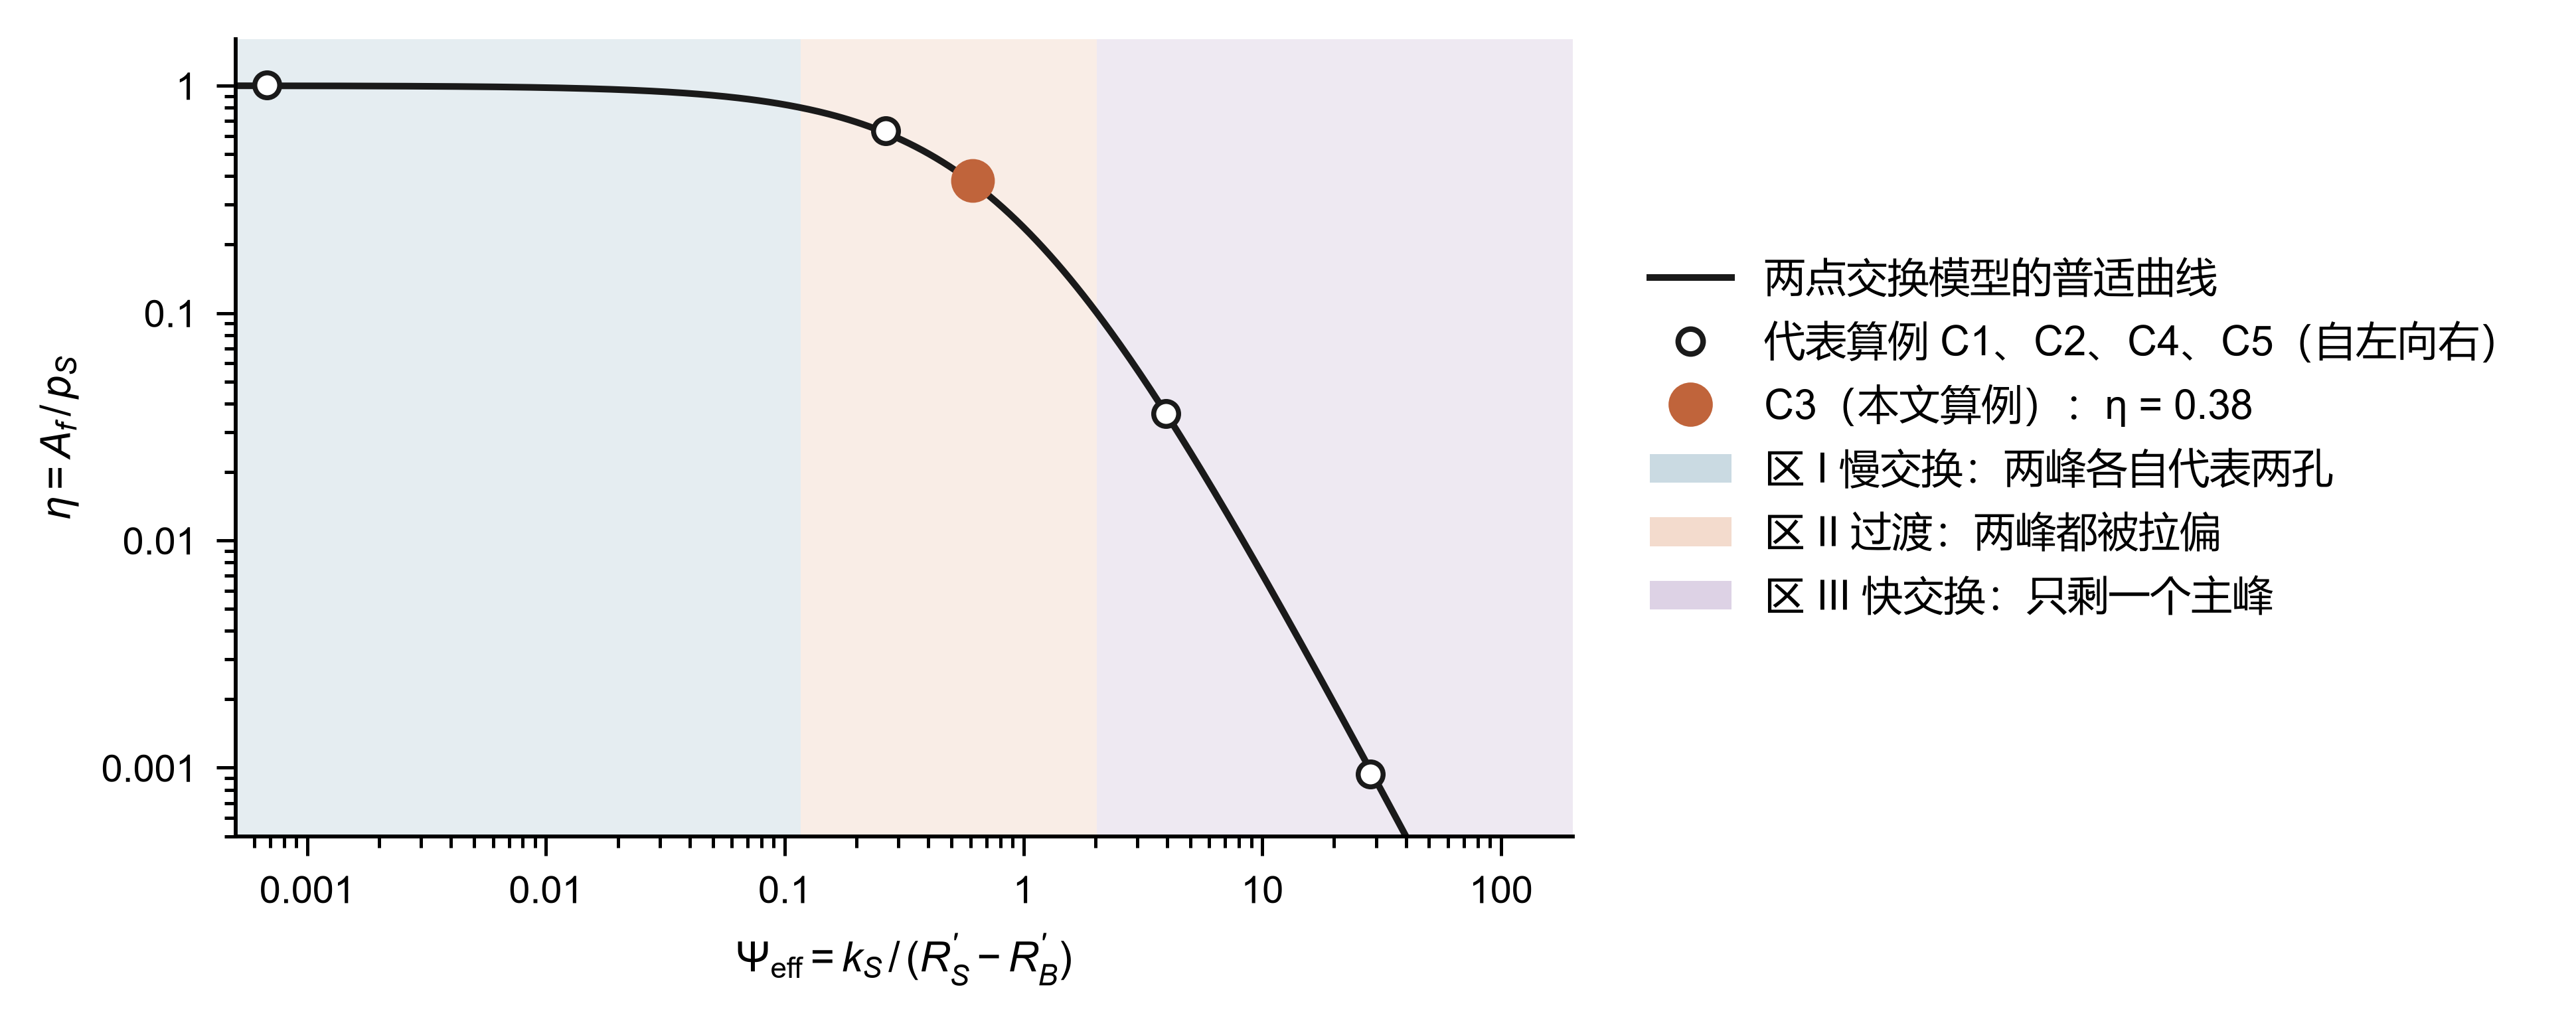
\includegraphics[width=0.86\textwidth]{fig_c3_regime.png}
\caption{C3 在“交换强弱”标尺上的位置。横轴为有效交换数 $\Peff$（交换快慢 / 两孔弛豫快慢之差），纵轴为小孔信号保留比 $\eta=A_f/p_S$（小峰面积 / 小孔应有面积）。
黑线是两点交换模型的普适曲线（怎么来的见第~\ref{sec:universal} 节），圆点是推导版中 5 个代表算例的精确模型值，C3（$\Peff=0.61$）位于过渡区。}
\label{fig:regime}
\end{figure}

%==========================================================================
\section{第四步：耦合以后，谱上的两个峰到底是什么}

\subsection{“模态”：整个体系的两种集体衰减方式}

\begin{intuit}
两孔连起来以后，不能再说“小孔一个 $T_2$、大孔一个 $T_2$”。整个体系变成两种\textbf{集体衰减方式}（模态），就像两个用弹簧连着的摆，有“同向摆”和“反向摆”两种模式。
\begin{itemize}[leftmargin=1.4em,itemsep=1pt]
\item \textbf{慢模态（主峰）= “平均磁化”的衰减}：两孔同涨同落，以大孔为主。
\item \textbf{快模态（小峰）= “两孔之间差别”的消失}：小孔比平均水平多出来的那部分磁化在消失。
这个差别有两条消失途径：小孔自己消磁快，再加上交换把差别“抹平”。两条路叠加，所以\textbf{快模态比小孔自身还快}。
\end{itemize}
\end{intuit}

\begin{formula}
\begin{equation}
\lambda_{f,s}=\frac{a+d\pm\sqrt{(a-d)^2+4k_Sk_B}}{2},\qquad a=R'_S+k_S,\quad d=R'_B+k_B,\qquad T_{2,f}=\frac{1}{\lambda_f},\ T_{2,s}=\frac{1}{\lambda_s}.
\end{equation}
\begin{itemize}[leftmargin=1.4em,itemsep=1pt]
\item $a$：小孔里一份磁化“离开”的总速率 = 被消磁（$R'_S$）+ 被搬走（$k_S$）。$d$ 是大孔的同一个量。
\item 根号项：交换让两个速率“互相推开”，快的更快、慢的更慢。没有交换（$k=0$）时，$\lambda_f=R'_S$、$\lambda_s=R'_B$，回到两个独立的孔。
\item 这是“两个相互影响的量”的标准解法（与求两个耦合摆的两种频率是同一类问题），不必推导。
\end{itemize}
\textbf{实用近似}：$\lambda_f\approx a=R'_S+k_S$，即“小峰的 $1/T_2$ $\approx$ 小孔自身（含下水道）+ 搬家速率”。
\end{formula}

\begin{numbers}
\begin{itemize}[leftmargin=1.4em,itemsep=1pt]
\item $a=3.172\times10^{-3}+1.404\times10^{-3}=4.577\times10^{-3}\pms$，$d=8.86\times10^{-4}+8.8\times10^{-5}=9.74\times10^{-4}\pms$。
\item 根号项 $=3.671\times10^{-3}$，于是 $\lambda_f=(5.550+3.671)/2\times10^{-3}=4.611\times10^{-3}\pms$，\textbf{$T_{2,f}=217\ms$}；
$\lambda_s=(5.550-3.671)/2\times10^{-3}=9.40\times10^{-4}\pms$，\textbf{$T_{2,s}=1064\ms$}。
\item 实用近似：$1/a=218\ms$，与 217\ms 几乎相同。
\end{itemize}
\end{numbers}

\subsection{两个峰被拉偏了多少——一步一步看}

\begin{table}[H]
\centering\small
\caption{C3 的两个峰从“孤立孔”到“实测”的变化。半径由孤立孔尺子 \eqref{eq:ruler} 换算；“手算”指本文的简化模型，“精确模型”指推导版的孔–喉–孔一维模型，“模拟 + NNLS”为全二维模拟的反演结果。}
\label{tab:shift}
\begin{tabular}{@{}l c c c c@{}}
\toprule
 & \multicolumn{2}{c}{小峰（小孔）} & \multicolumn{2}{c}{主峰（大孔）} \\
\cmidrule(lr){2-3}\cmidrule(lr){4-5}
 & $T_2$ (ms) & 读出半径 (\si{\micro m}) & $T_2$ (ms) & 读出半径 (\si{\micro m}) \\
\midrule
孤立孔 & 441 & 5.16 & 1206 & 20.16 \\
+ 喉道下水道 & 315 & 3.52 & 1129 & 18.10 \\
+ 下水道 + 交换（手算） & 217 & 2.34 & 1064 & 16.49 \\
精确模型 & 229 & 2.48 & 1070 & 16.63 \\
模拟 + NNLS & 215 & 2.31 & 1087 & 17.04 \\
\midrule
真实半径 & & 5 & & 20 \\
\bottomrule
\end{tabular}
\end{table}

\begin{figure}[H]
\centering
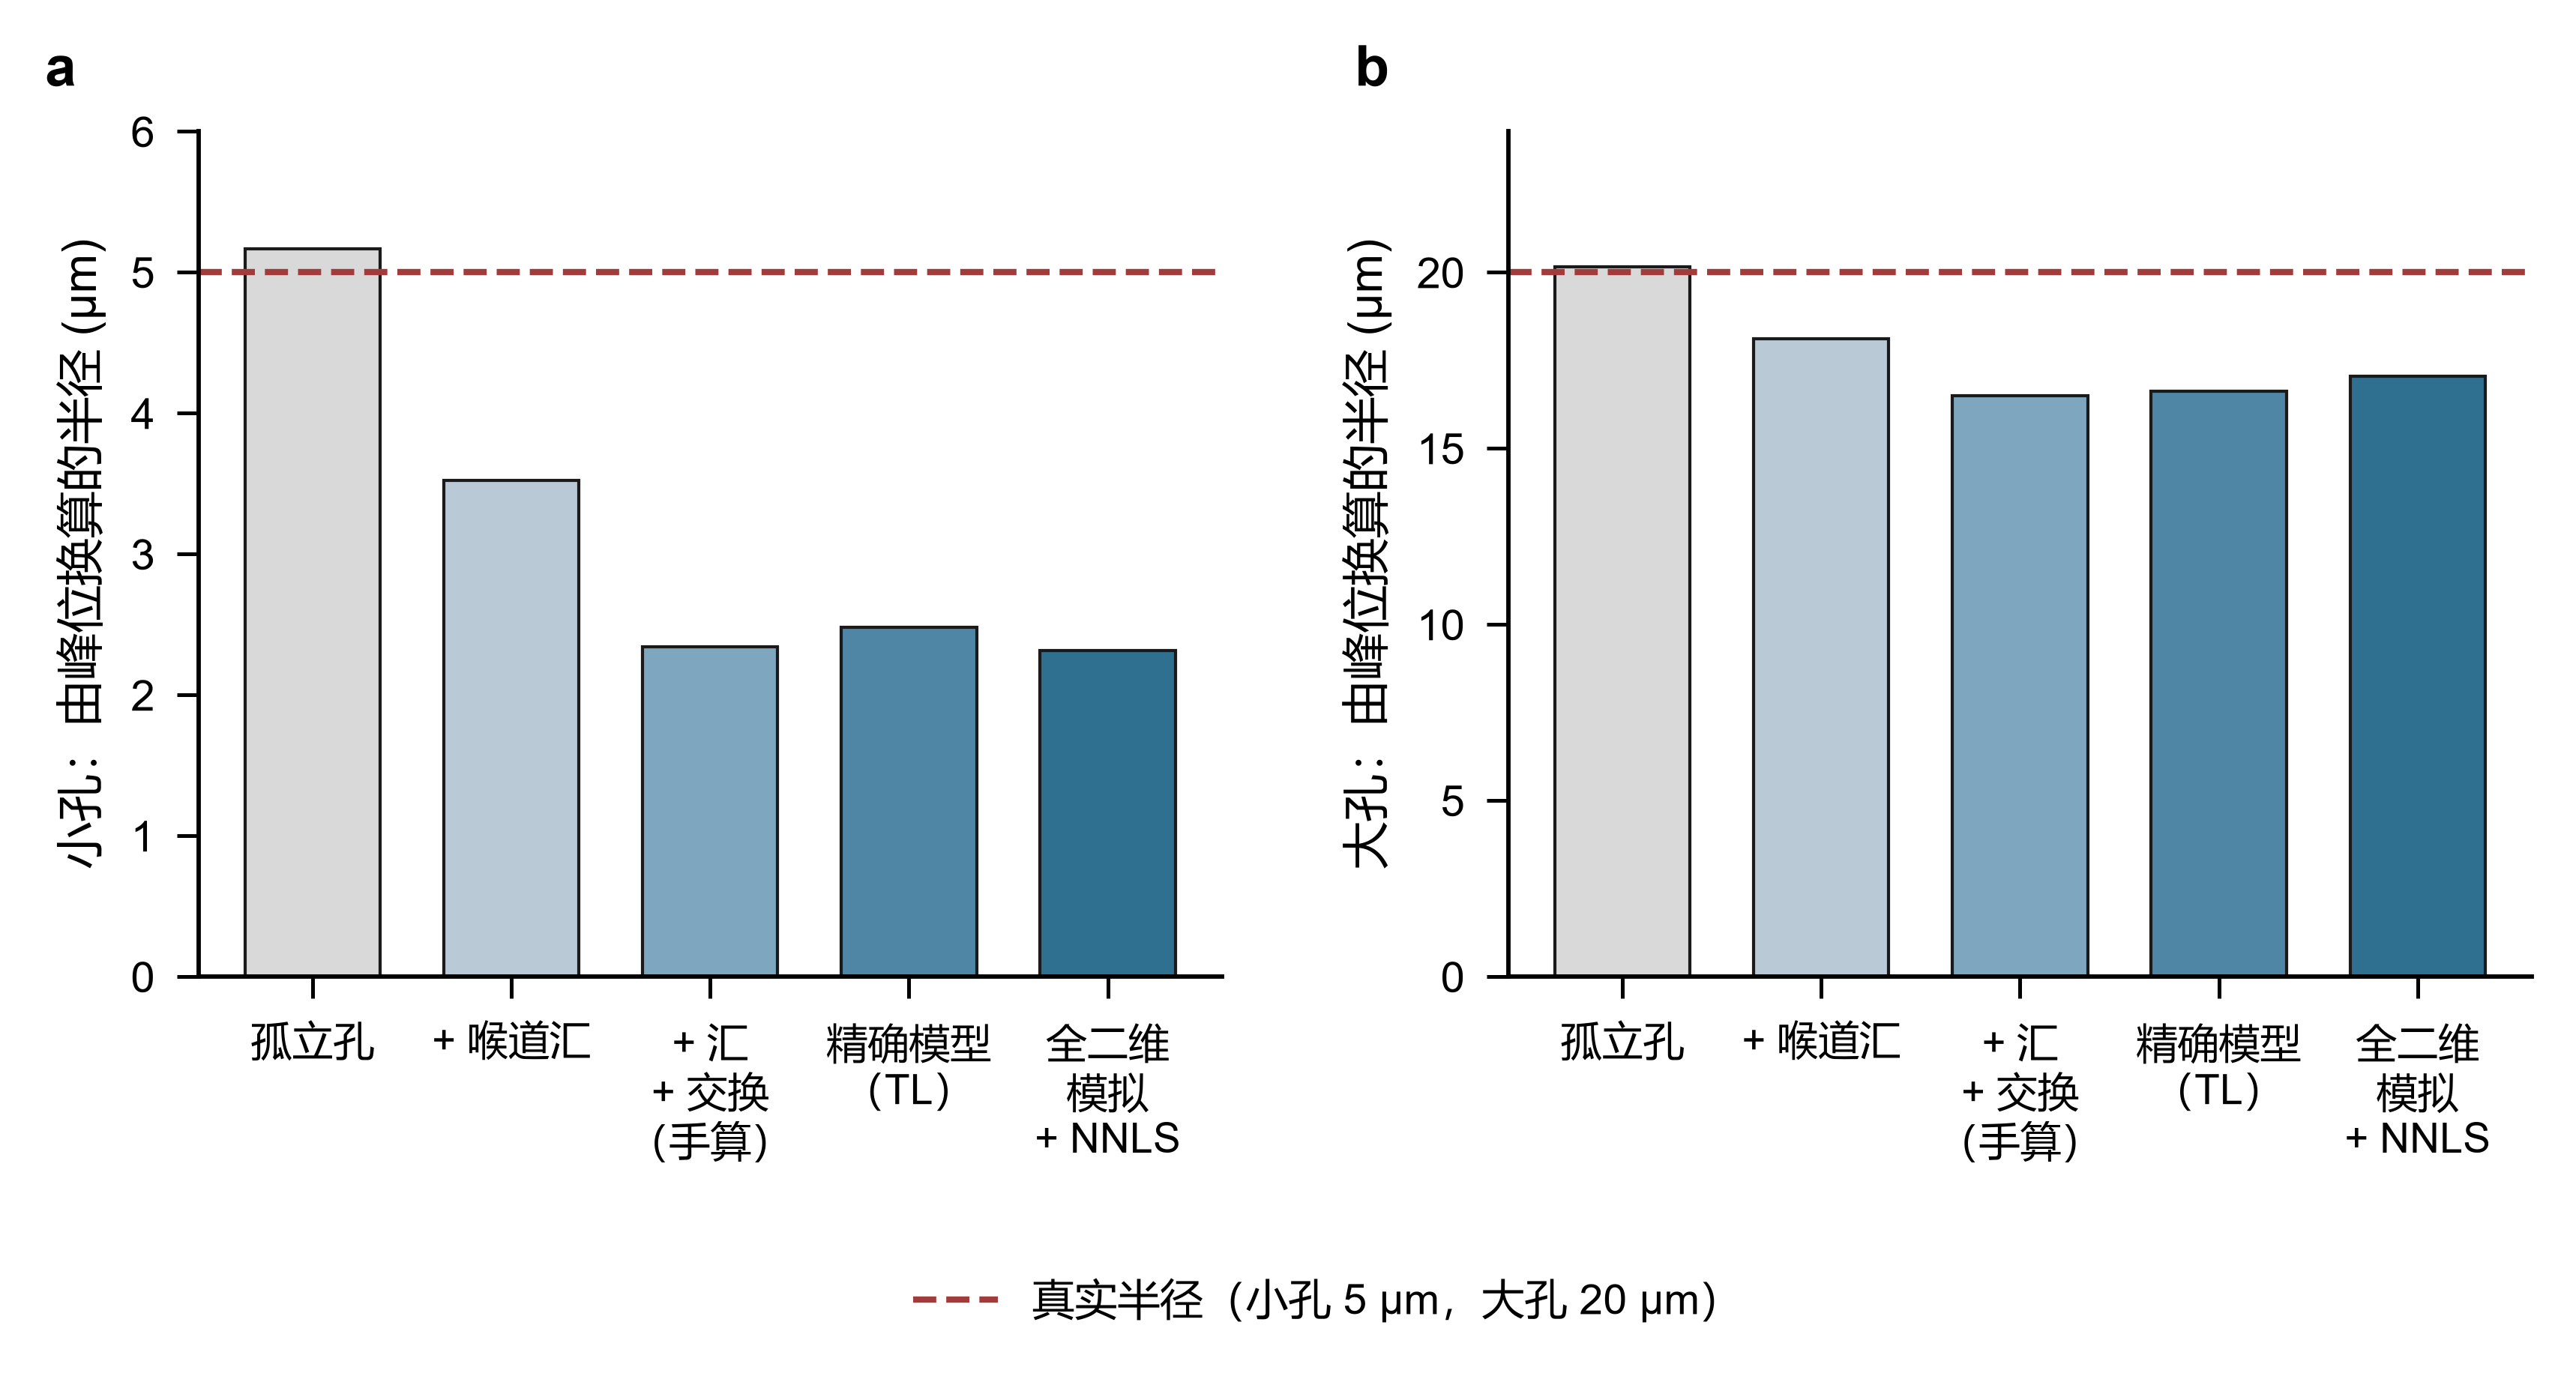
\includegraphics[width=\textwidth]{fig_c3_peak_shift.png}
\caption{如果把每个峰都当作“孤立孔”去换算，读出的半径如何一步步偏离真值（红色虚线）。(a) 小孔；(b) 大孔。数值见表~\ref{tab:shift}。}
\label{fig:shift}
\end{figure}

\begin{takeaway}
\begin{itemize}[leftmargin=1.4em,itemsep=1pt]
\item 小孔峰：441 → 315\ms（下水道）→ 217\ms（交换），读出的半径从 5.2 掉到 2.3\um，\textbf{低估一半以上}。两步的贡献大致相当。
\item 主峰：1206 → 1129 → 1064\ms。大孔的水“借用”了小孔和喉道的消磁能力，\textbf{大孔也被低估约 15\%}。
\item 主峰的位置介于“大孔单独”（含下水道，1129\ms）和“两孔完全混合”（980\ms，见下一节）之间，大约走了 40\% 的路——这正是“混合进行到一半”的另一种说法。
\item 手算（217\ms）与精确模型（229\ms）相差约 5\%，来自简化模型的近似；它不改变上面的定性结论。（这一组算例中，NNLS 的小峰位置恰好更接近手算值。）
\end{itemize}
\end{takeaway}

\subsection{小峰为什么变“矮”了——用两句话算出峰面积}
\label{sec:area}

\begin{intuit}
不需要解方程，只用两个简单事实：
\begin{enumerate}[leftmargin=1.6em,itemsep=1pt]
\item 两个峰的面积加起来等于全部的水：$A_f+A_s=1$。
\item 在 $t=0$ 那一瞬间，两孔的磁化都是满的、没有差别，所以\textbf{交换还没开始起作用}（没有差别就没有扩散）。
此时整个体系衰减的快慢只取决于“各孔有多少墙（含下水道）”，按面积加权平均即可。
\end{enumerate}
\end{intuit}

\begin{formula}
\begin{equation}
A_f+A_s=1,\qquad A_f\lambda_f+A_s\lambda_s=\bar R'=p_SR'_S+p_BR'_B
\quad\Longrightarrow\quad A_f=\frac{\bar R'-\lambda_s}{\lambda_f-\lambda_s},\qquad \eta=\frac{A_f}{p_S}.
\end{equation}
$\eta$ 是小孔信号的\textbf{保留比}：小峰面积占“小孔应有面积 $p_S$”的比例。没有耦合时 $\eta=1$。
\end{formula}

\begin{numbers}
$\bar R'=0.0588\times3.172\times10^{-3}+0.9412\times8.86\times10^{-4}=1.020\times10^{-3}\pms$（即“完全混合”时的 $T_2=980\ms$）。
\[
A_f=\frac{1.020-0.940}{4.611-0.940}=\frac{0.081}{3.671}=0.0220,\qquad \eta=\frac{0.0220}{0.0588}=0.37.
\]
精确模型 $A_f=0.0225$（$\eta=0.38$），模拟 + NNLS 的小峰面积 0.0231（$\eta=0.39$）。
\end{numbers}

\begin{figure}[H]
\centering
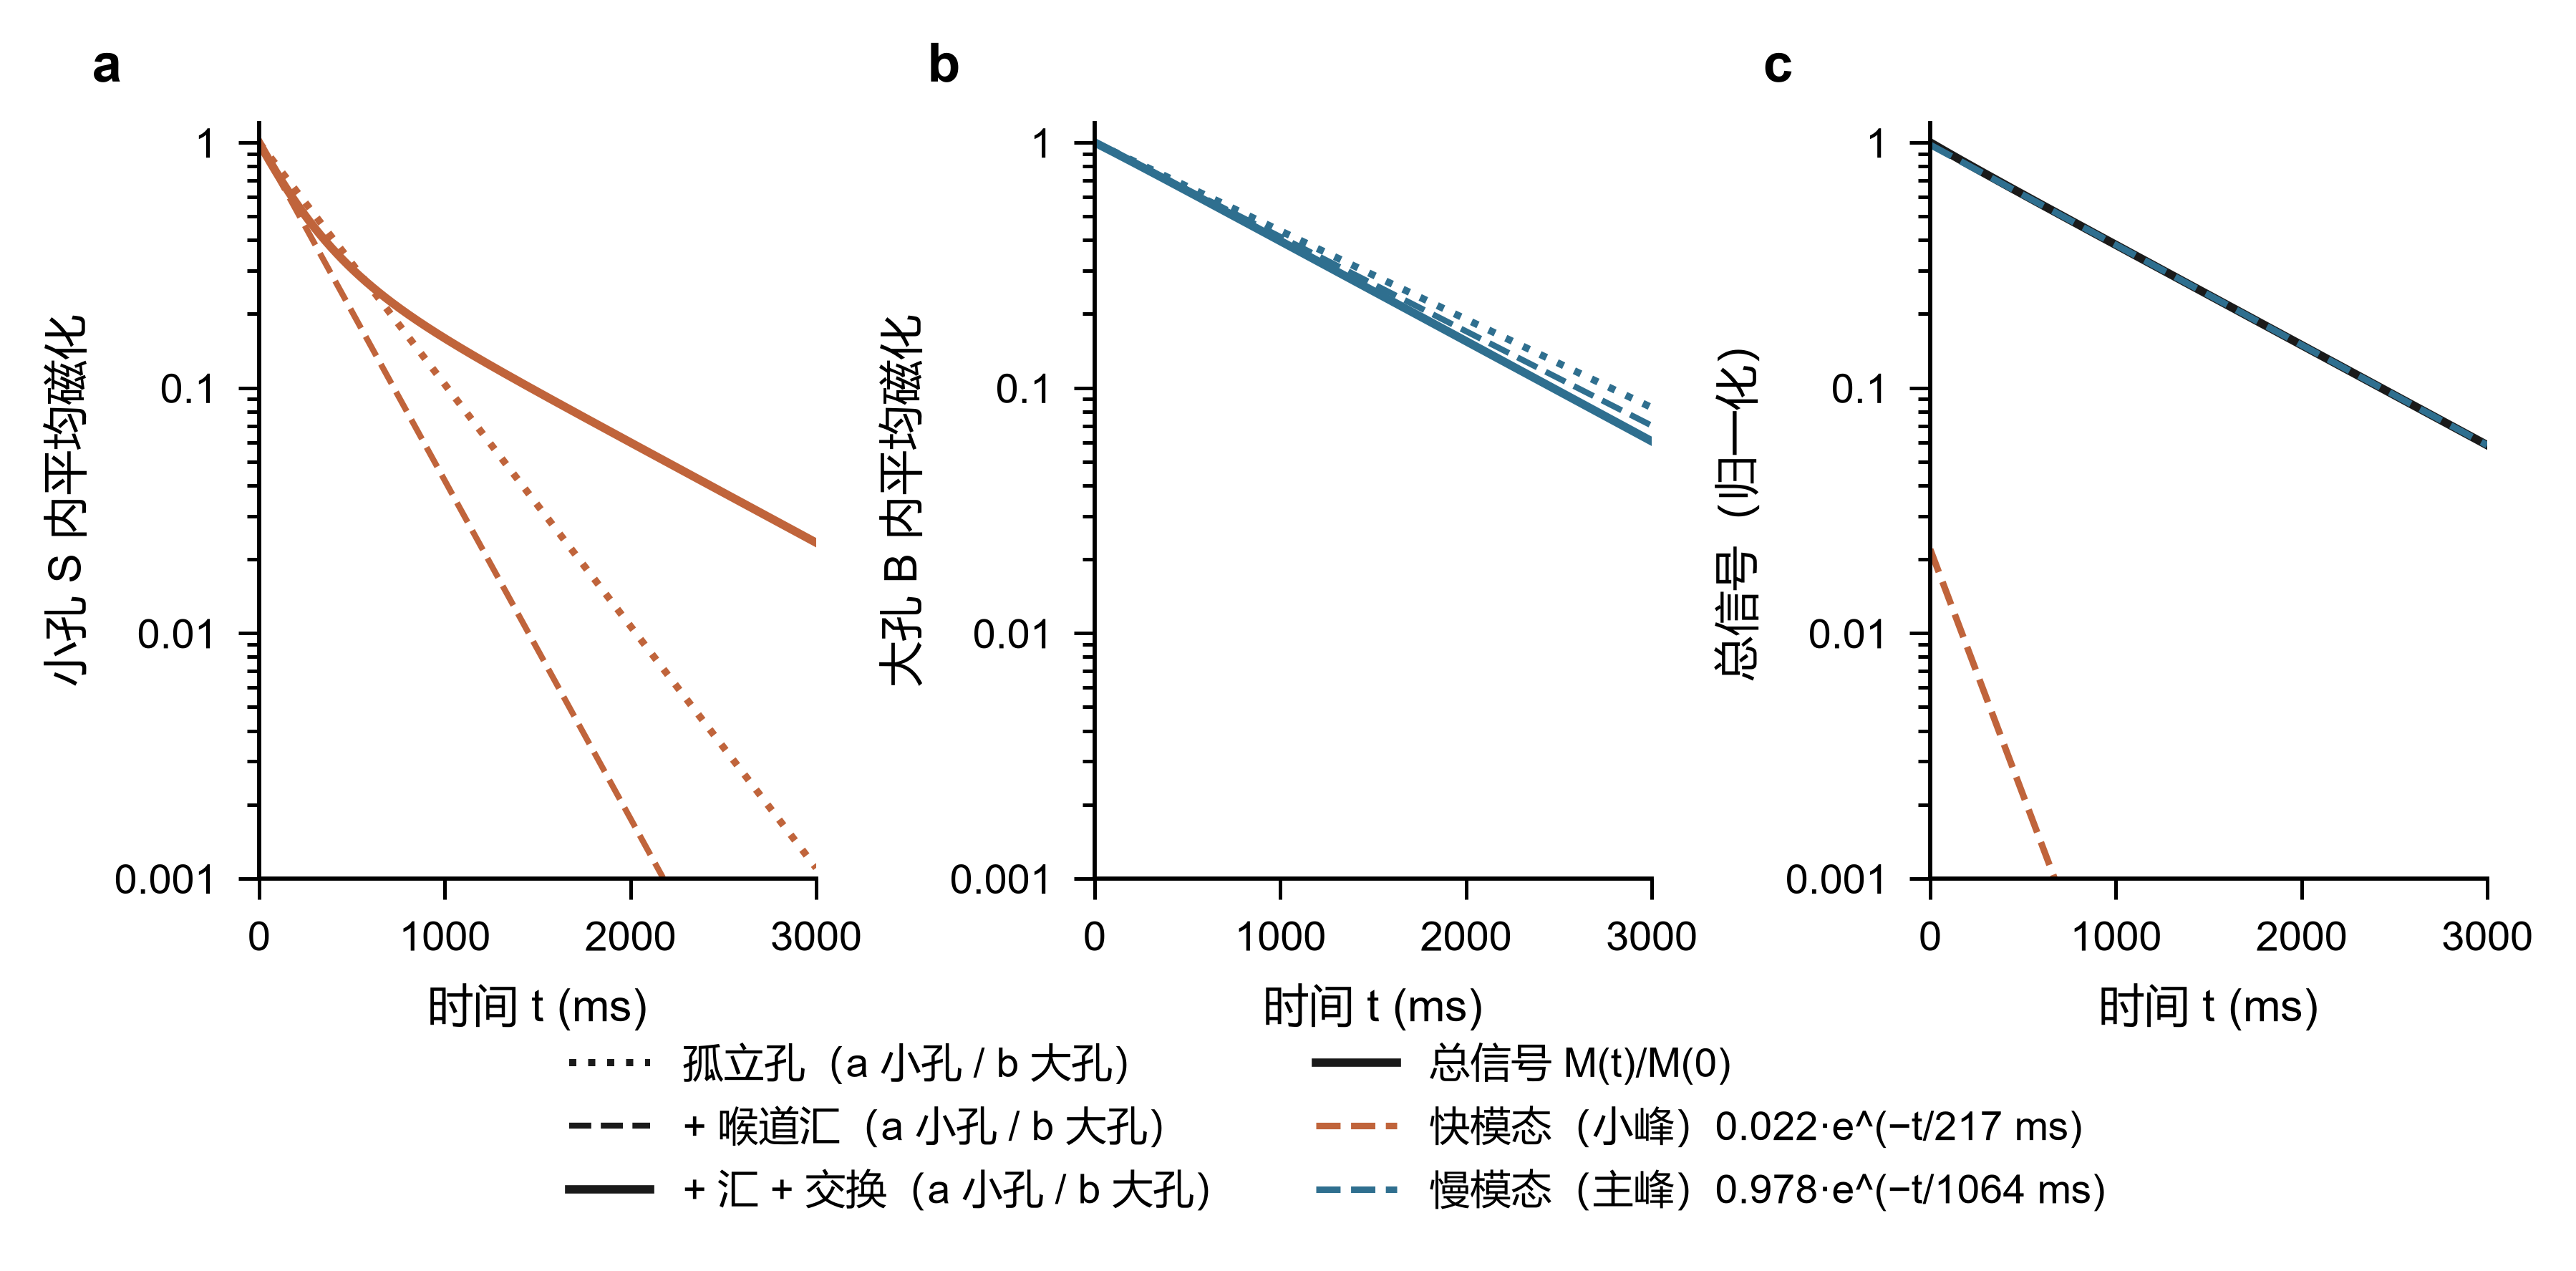
\includegraphics[width=\textwidth]{fig_c3_time_domain.png}
\caption{在时间域里看耦合（简化模型）。(a) 小孔内平均磁化：孤立时（点线）、只加下水道（虚线）、再加交换（实线）。
实线先快速下降，约 600\ms 后拐弯，改为跟着大孔的速度慢慢衰减——小孔在被大孔“输血”。
(b) 大孔内平均磁化：三条线很接近，大孔只被略微拉快。(c) 总信号及其两个模态分量：快模态（小峰）只占 0.022。}
\label{fig:time}
\end{figure}

\begin{takeaway}
\begin{itemize}[leftmargin=1.4em,itemsep=1pt]
\item 小孔 100 份水的信号里，只有约 \textbf{37 份留在小峰}，其余约 63 份\textbf{并入了主峰}。
\item 时间域图~\ref{fig:time}(a) 给出直观原因：小孔里的磁化不断被大孔补充，后期它跟着大孔一起以 1064\ms 衰减，这部分信号在谱上自然被算进主峰。
（定量上，小孔磁化约 61\% 按快模态衰减、39\% 按慢模态衰减；快模态在大孔里还带一个很小的反向分量，所以小峰面积比 61\% 对应的值还要小，最终 $\eta=0.37$。）
\item 因此\textbf{小峰面积 $\neq$ 小孔体积}。用小峰面积估计小孔含量，会把小孔低估一半以上。
\end{itemize}
\end{takeaway}

\subsection{回头看图~\ref{fig:regime}：普适曲线是怎么来的}
\label{sec:universal}

现在已经有了全部工具，可以回答：图~\ref{fig:regime} 里那条黑色的“普适曲线”是怎么画出来的，为什么不同喉道的算例都落在同一条线上。

\begin{intuit}
曲线上的每一个点都是一次计算：固定小孔占比 $p_S$，只改变“走廊”的强弱，用上面的三个公式（$\lambda_f$、$\lambda_s$、$A_f$）算出 $\eta$，再把 $(\Peff,\eta)$ 画到图上。

之所以叫“普适”，是因为\textbf{不管两孔的消磁速率具体是多少，只要 $\Peff$ 和 $p_S$ 相同，算出的 $\eta$ 就完全相同}。原因只有两条，都很直观：
\begin{enumerate}[leftmargin=1.6em,itemsep=1pt]
\item \textbf{去掉公共背景（平移）}：两个孔都至少以 $R'_B$ 的速率衰减，这是大家共有的“背景”。把整条信号乘以 $e^{R'_Bt}$ 扣掉这个背景，
两个峰的相对大小不变；真正起作用的只是小孔“多出来”的那部分速率 $R'_S-R'_B$。
\item \textbf{换一只钟（缩放）}：用 $1/(R'_S-R'_B)$ 作为时间单位。峰的面积不会因为换了钟而改变。
\end{enumerate}
做完这两步，所有速率都变成了“以 $R'_S-R'_B$ 为单位”的数：小孔多出来的速率 $=1$，小孔的搬家速率 $=\Peff$，大孔的搬家速率 $=\Peff\,p_S/p_B$。
整个问题只剩下 $\Peff$ 和 $p_S$ 两个数，所以 $\eta$ 只能是它俩的函数。

\textbf{工程类比——雷诺数与 Moody 图}：不同管径、流速、流体，只要雷诺数 $Re$ 相同，流动状态就相同，摩阻系数可以画成一条随 $Re$ 变化的曲线。
$\Peff$ 就是这里的“雷诺数”，图~\ref{fig:regime} 就是这里的“Moody 图”。
\end{intuit}

\begin{formula}[：把上面三个公式写成无量纲形式]
把上面“平移、换钟”两步代入 $\lambda_{f,s}$ 和 $A_f$ 的公式（带星号的量都以 $R'_S-R'_B$ 为单位，并已扣除 $R'_B$）：
\begin{align}
a^*&=1+\Peff,\qquad d^*=\Peff\,\frac{p_S}{p_B},\qquad \bar R^{\prime *}=p_S, \notag\\
\lambda^*_{f,s}&=\frac{a^*+d^*\pm\sqrt{(a^*-d^*)^2+4\,\Peff\,d^*}}{2}, \notag\\
\eta(\Peff;\,p_S)&=\frac{p_S-\lambda^*_s}{p_S\,(\lambda^*_f-\lambda^*_s)} .
\label{eq:universal}
\end{align}
式 \eqref{eq:universal} 里只出现 $\Peff$ 和 $p_S$。固定 $p_S$，让 $\Peff$ 从 0.001 扫到 100，算出一串 $\eta$ 连成线，就是图~\ref{fig:regime} 的黑线
（\texttt{make\_figures.py} 中的 \texttt{eta\_two\_site()}）。

两端的形状也可以直接读出来：
\begin{itemize}[leftmargin=1.4em,itemsep=1pt]
\item $\Peff\to0$（不交换）：$\lambda^*_f\to1$、$\lambda^*_s\to0$，$\eta\to1$，小峰完整保留——曲线左边的平台。
\item $\Peff\gg1$（强交换）：$\eta\approx p_B^3/\Peff^2$。$\Peff$ 每增大 10 倍，$\eta$ 降为 1/100——曲线右边在双对数坐标里是斜率为 $-2$ 的直线。
\end{itemize}
\end{formula}

\begin{numbers}
C3：$\Peff=0.614$，$p_S=0.0588$，$p_B=0.9412$。
\[
a^*=1.614,\quad d^*=0.614\times\frac{0.0588}{0.9412}=0.0384,\quad
\sqrt{(1.614-0.0384)^2+4\times0.614\times0.0384}=1.606,
\]
\[
\lambda^*_f=\frac{1.653+1.606}{2}=1.629,\qquad \lambda^*_s=\frac{1.653-1.606}{2}=0.0236,
\]
\[
\eta=\frac{0.0588-0.0236}{0.0588\times(1.629-0.0236)}=0.37 .
\]
与第~\ref{sec:area} 节用真实速率算出的 $\eta=0.37$ 完全相同——换了单位，结果不变。曲线上其他几个点：
\begin{center}\small
\begin{tabular}{@{}lccccc@{}}
\toprule
$\Peff$ & 0.01 & 0.1 & 0.61（C3） & 2 & 10 \\
$\eta$ & 0.98 & 0.83 & 0.37 & 0.10 & 0.0071 \\
\bottomrule
\end{tabular}
\end{center}
$\eta=0.8$ 和 $\eta=0.1$ 分别对应 $\Peff\approx0.12$ 和 $\Peff\approx2.0$，这就是图~\ref{fig:regime} 中三个区的分界。
在 $\Peff=10$ 处，强交换近似给出 $p_B^3/\Peff^2=0.0083$，与精确值 0.0071 已比较接近。
\end{numbers}

\begin{figure}[H]
\centering
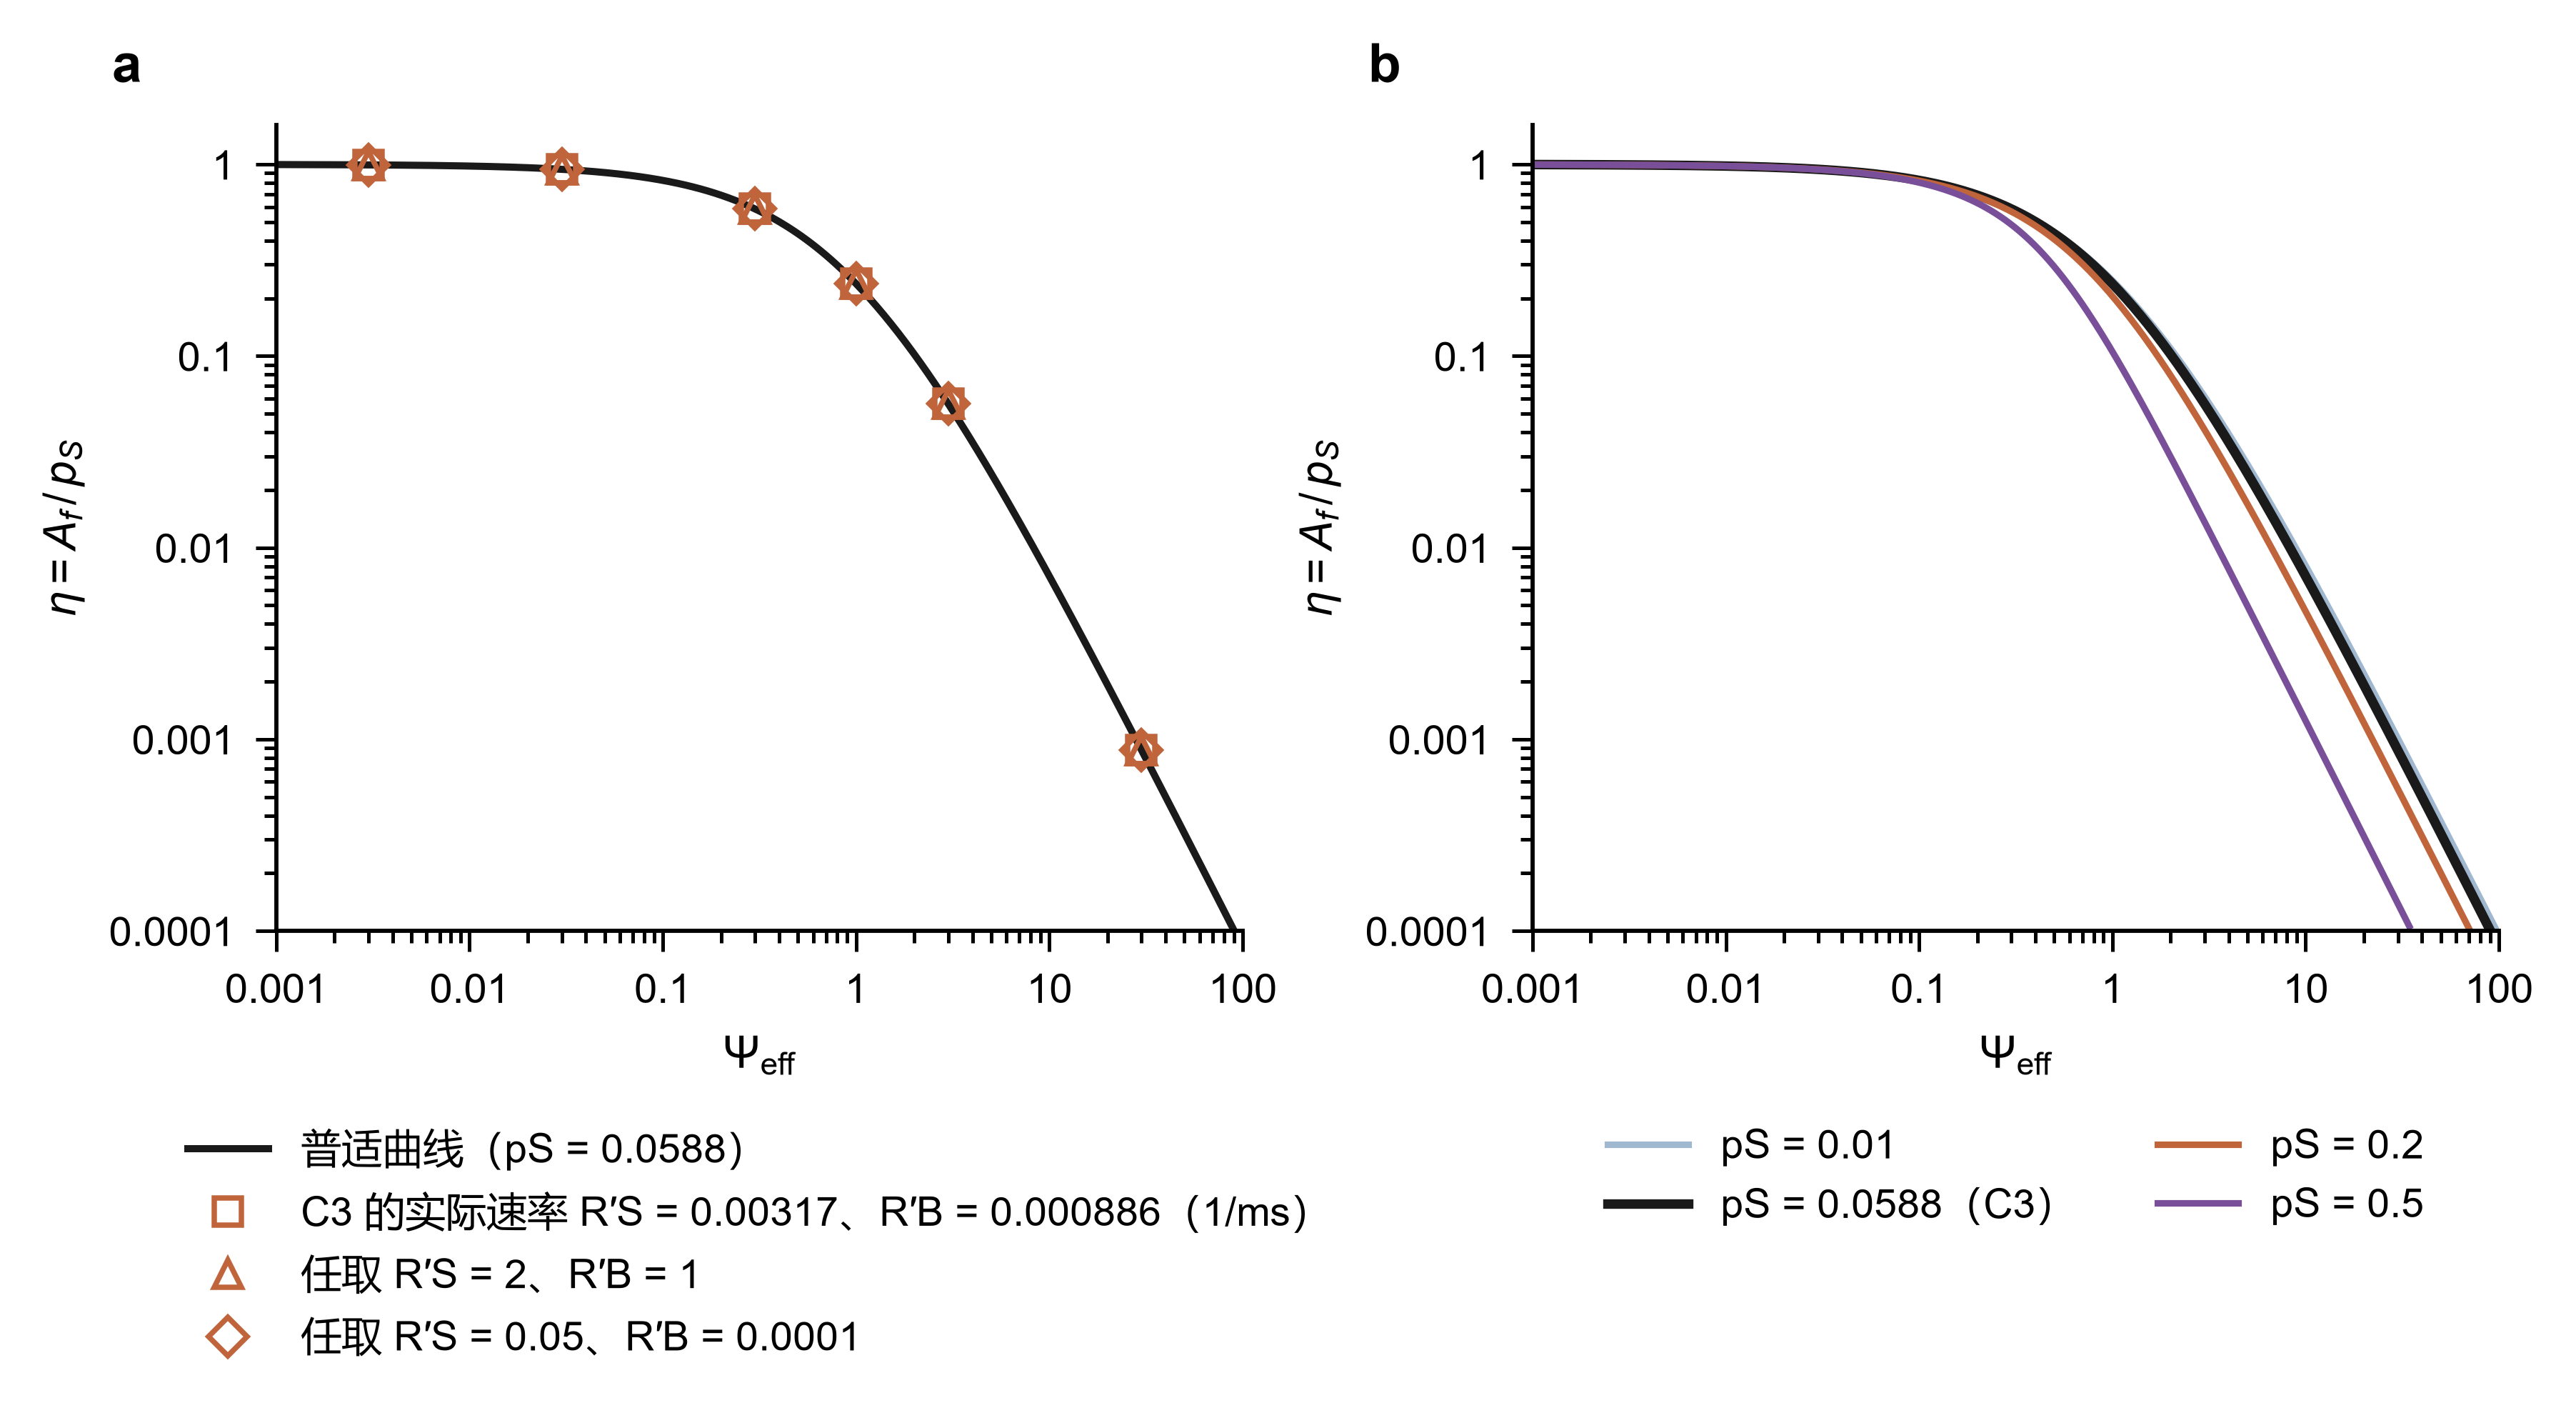
\includegraphics[width=\textwidth]{fig_c3_universal.png}
\caption{普适曲线的检验。(a) 三组相差很大的消磁速率（C3 的实际速率，以及两组任意取值）在相同 $\Peff$ 下算出的 $\eta$ 完全重合在同一条曲线上：只有 $\Peff$ 起作用。
(b) 改变小孔占比 $p_S$ 时曲线会移动：$p_S$ 很小时（0.01 与 C3 的 0.0588）几乎重合；$p_S$ 越大，同样的 $\Peff$ 下小峰丢失得越多。}
\label{fig:universal}
\end{figure}

\begin{takeaway}
\begin{itemize}[leftmargin=1.4em,itemsep=1pt]
\item 推导版的 20 个算例孔的几何相同，$p_S$ 都是 0.0588，所以可以用\textbf{同一条曲线}判断；喉道的不同（宽、长）全部体现在 $\Peff$ 这一个数上。
\item 图~\ref{fig:regime} 里的圆点不是这条曲线算出来的，而是推导版精确模型（孔–喉–孔一维模型）的结果，所以只是落在曲线\emph{附近}：
C3 的精确值 0.38，曲线值 0.37，差别来自喉道的准静态近似。
\item 换一种样品（小孔占比不同），要用对应 $p_S$ 的曲线（图~\ref{fig:universal}b），区的分界也会随之移动。
\item 这条曲线建立在两个假设上：每个孔内部磁化均匀（第一步），喉道满足准静态收支平衡（第~\ref{sec:throat-balance} 节）。
\end{itemize}
\end{takeaway}

%==========================================================================
\section{第五步：反算——直接换算为什么错，怎样纠正}

\subsection{三种做法的对比}

\begin{table}[H]
\centering\small
\caption{C3 的三种反算做法（输入均为模拟 + NNLS 的谱，SNR 1000）。}
\label{tab:back}
\begin{tabular}{@{}p{3.2cm} p{6.6cm} c c@{}}
\toprule
做法 & 思路 & 小孔 (\si{\micro m}) & 大孔 (\si{\micro m}) \\
\midrule
A 直接换算 & 每个峰按孤立孔尺子 \eqref{eq:ruler} 换算 & 2.31 & 17.04 \\
B 面积比 & 主峰换算大孔；小孔由两峰面积比 $r_S=r_B\sqrt{f_S/f_B}$ 推出 & 2.62 & 17.04 \\
D 已知喉道的模型反演 & 已知 $w$、$L$，调整 $(r_S,r_B)$ 直到模型给出的两峰位置和面积与实测一致 & \textbf{4.84} & \textbf{19.61} \\
\midrule
真实值 & & 5 & 20 \\
\bottomrule
\end{tabular}
\end{table}

\begin{numbers}
\begin{itemize}[leftmargin=1.4em,itemsep=1pt]
\item A：$r_S=0.01/(1/214.79-1/3000)=2.31\um$，$r_B=0.01/(1/1086.72-1/3000)=17.04\um$（$0.01=2\rho_2$）。
\item B：二维圆孔面积 $\propto r^2$，若小峰面积分数 $f_S$ 等于小孔面积分数，则 $r_S=r_B\sqrt{f_S/f_B}=17.04\times\sqrt{0.0231/0.9769}=2.62\um$。
它失败的原因正是上一节的 $\eta=0.39$：小峰面积少了六成，开平方后半径仍少了约四成。
\item D：给定 $w=1\um$、$L=15\um$，模型能完整重复本文第二到第四步的计算；调整 $(r_S,r_B)$ 使模型预测与实测的 $(T_{2,f},T_{2,s},A_f)$ 最接近，得到 4.84 和 19.61\um。
如果输入的是精确模型自己的峰（不含 NNLS 误差），会准确回到 5.00 和 20.00\um，说明剩余 2--3\% 的误差来自 NNLS 反演把峰“抹宽”。
\end{itemize}
\end{numbers}

\begin{intuit}[：做法 D 像是“扣皮重”]
称一箱货，读数里包含了箱子的重量。只要知道箱子多重，就能扣掉得到净重。
在这里，“读数”是谱上的两个峰，“箱子”是喉道造成的下水道和交换偏移；只要知道喉道尺寸，就能把偏移算出来、扣除。
\textbf{不知道喉道尺寸时，这一步就做不了}：同样的谱可以由“孔小但交换弱”或“孔大但交换强”等多种组合产生。
\end{intuit}

\subsection{拿到一条实测谱时的实用检查清单}

\begin{enumerate}[leftmargin=1.6em,itemsep=2pt]
\item \textbf{比面积}：如果小峰面积明显小于 CT 估计的小孔体积分数，说明存在耦合（$\eta<1$），不能直接用面积估计小孔含量。
\item \textbf{估交换强弱}：用 CT 得到的喉道宽、长和孔径，估算 $\Psi=(Dw/L)/[A_S(R_S-R_B)]$（二维形式），判断大致属于哪个区。
\item \textbf{按区处理}：区 I（$\Psi$ 远小于 0.1）两峰面积可信，主峰可直接换算大孔，小孔用面积比（做法 B）推出——
小峰\emph{位置}仍可能被下水道拉偏（推导版 C1 中直接换算小孔只得 3.5\um，做法 B 得 4.3\um）；
区 II 需要做法 D 那样的模型校正；区 III 只能报告一个等效半径，并说明小孔可能被隐藏。
\item \textbf{别忘了下水道}：即使两孔交换很弱，细喉道仍会把相邻小孔的峰往短 $T_2$ 方向拉。
\item \textbf{三维样品}：上面的数字都来自二维模型；三维圆柱形喉道的“走廊”和“下水道”都比二维窄缝弱，$\Psi$ 的几何因子需要重新计算。
\end{enumerate}

%==========================================================================
\section{本算例的知识点汇总}

\begin{enumerate}[leftmargin=1.6em,itemsep=2pt]
\item 孤立孔的 $1/T_2$ 由“每份水对应多少墙”决定（$\rho_2P/A$），所以小孔快、大孔慢；反过来就是读孔径的尺子 \eqref{eq:ruler}。
\item 这把尺子只对孤立孔准确；孔被喉道连起来后，读数系统性偏小。
\item 喉道里两壁很近，水约 97\ms 就消磁，所以喉道同时是“走廊”（交换）和“下水道”（汇）。
\item $qL$ = 喉道长度 / 分子在喉道里的寿命行程，决定喉道偏“走廊”还是偏“下水道”。C3 的 $qL=1.08$，两者都重要。
\item 下水道对小孔影响大（每份水分到的漏口多）：C3 中仅此一项就把小孔 $T_2$ 从 441 压到 315\ms。
\item $\Peff$ = 搬家速率 / 消磁速率之差，决定是“两个峰”还是“一个平均峰”。C3 的 $\Peff=0.61$，处在过渡区。
\item 耦合后谱上的峰是整个体系的“模态”，而不是某一个孔：小峰是“差别在消失”，主峰是“平均在衰减”。
\item 小峰的 $1/T_2$ $\approx$ 小孔自身（含下水道）+ 搬家速率，所以比孤立小孔更快：C3 为 217\ms。
\item 小峰保留比 $\eta$ 只取决于 $\Peff$ 和小孔占比 $p_S$，与两孔消磁速率的具体数值无关，所以能画成一条普适曲线（类似雷诺数与 Moody 图）。
\item 小峰面积只保留了小孔信号的 37\%，其余并入主峰，所以小峰面积 $\neq$ 小孔体积。
\item 主峰也被拉短（1206 → 1064--1087\ms），大孔被低估约 15\%。
\item 已知喉道尺寸时，可以用模型把这些偏移“扣除”（C3：4.84 / 19.61\um）；不知道时，只能给出范围或等效尺寸。
\end{enumerate}

\section{常见误区}

\begin{pitfall}[误区 1：“谱上只有一个峰，就说明只有一种孔”]
在区 III，小孔的信号几乎全部并入主峰（推导版 C5 中 $\eta<0.1\%$）。一个峰只说明交换很强，不说明小孔不存在。
\end{pitfall}
\begin{pitfall}[误区 2：“小峰偏左，说明小孔比 CT 看到的更小”]
C3 中小孔真实半径是 5\um，峰却读成 2.3\um。偏左来自下水道和交换两种耦合效应，不是孔更小。
\end{pitfall}
\begin{pitfall}[误区 3：“小峰面积就是小孔的体积分数”]
C3 中小峰面积 2.3\%，小孔实际占 5.9\%。只有在区 I（$\eta\approx1$）才近似成立。
\end{pitfall}
\begin{pitfall}[误区 4：“大孔离喉道远，不受影响”]
大孔峰同样被拉短约 10\%，直接换算会低估大孔约 15\%。
\end{pitfall}

\section{符号速查表}

\begin{table}[H]
\centering\footnotesize\renewcommand{\arraystretch}{0.95}
\begin{tabular}{@{}l l p{6.2cm} l@{}}
\toprule
符号 & 名称 & 通俗含义 & C3 数值 \\
\midrule
$R_S,R_B$ & 孔自身消磁速率 & 孤立孔的 $1/T_2$ & $2.27\times10^{-3}$，$8.29\times10^{-4}\pms$ \\
$R_t$ & 喉道消磁速率 & 喉道里水的 $1/T_2$ & $0.0103\pms$（97\ms） \\
$\ell=1/q$ & 寿命行程 & 分子在喉道里“活着”能走的距离 & 13.9\um \\
$qL$ & 喉道性格数 & 喉道长度 / 寿命行程 & 1.08 \\
$G_x$ & 交换导纳 & 走廊的有效通过能力 & $0.110\,\si{\micro m^2/ms}$ \\
$G_s$ & 汇导纳 & 每个喉口的“漏磁”能力 & $0.0709\,\si{\micro m^2/ms}$ \\
$R'_S,R'_B$ & 含下水道的速率 & 孔自身 + 下水道 & $3.17\times10^{-3}$，$8.86\times10^{-4}\pms$ \\
$k_S,k_B$ & 搬家速率 & 每份水每 ms 换到另一孔的概率 & $1.40\times10^{-3}$，$8.8\times10^{-5}\pms$ \\
$\Peff$ & 有效交换数 & 搬家速率 / 消磁速率之差 & 0.61 \\
$T_{2,f},T_{2,s}$ & 两个模态的 $T_2$ & 小峰、主峰的位置 & 217，1064\ms（手算） \\
$\bar R'$ & 平均速率 & 两孔完全混合时的 $1/T_2$ & $1.02\times10^{-3}\pms$（980\ms） \\
$A_f$ & 快模态权重 & 小峰面积 & 0.022 \\
$\eta=A_f/p_S$ & 保留比 & 小峰面积 / 小孔应有面积 & 0.37 \\
\bottomrule
\end{tabular}
\end{table}

\noindent 想进一步了解：孔内快扩散与弛豫的经典分析见 \citet{BrownsteinTarr1979}；两点交换模型最早见 \citet{ZimmermanBrittin1957}；
岩石中微孔–宏孔扩散耦合的讨论见 \citet{AnandHirasaki2007}。

{\small
\begin{thebibliography}{3}
\setlength{\itemsep}{2pt}

\bibitem[Anand \& Hirasaki(2007)]{AnandHirasaki2007}
Anand, V., \& Hirasaki, G. J. (2007). Diffusional coupling between micro and macroporosity for NMR relaxation in sandstones and grainstones.
\emph{Petrophysics}, \emph{48}(4), 289--307.

\bibitem[Brownstein \& Tarr(1979)]{BrownsteinTarr1979}
Brownstein, K. R., \& Tarr, C. E. (1979). Importance of classical diffusion in NMR studies of water in biological cells.
\emph{Physical Review A}, \emph{19}(6), 2446--2453. \url{https://doi.org/10.1103/PhysRevA.19.2446}

\bibitem[Zimmerman \& Brittin(1957)]{ZimmermanBrittin1957}
Zimmerman, J. R., \& Brittin, W. E. (1957). Nuclear magnetic resonance studies in multiple phase systems: Lifetime of a water molecule
in an adsorbing phase on silica gel. \emph{The Journal of Physical Chemistry}, \emph{61}(10), 1328--1333. \url{https://doi.org/10.1021/j150556a015}
\end{thebibliography}
}

\end{document}
